\chapter{Differentialgleichungen}

Differentialgleichungen sind eines der wichtigsten Fundamente für die Beschreibung von Zusammenhängen in der Natur. Sie stellen einen Zusammenhang her zwischen einer Größe und ihrer Änderungsrate. In der klassischen Mechanik etwa stellt man sich die Frage, wie sich ein Körper und Einfluss einer Kraft bewegt. Die gesamte Bahn des Körpers anzugeben, ist nicht einfach. Einfacher ist es zu betrachten, was lokal zu einem konkreten Zeitpunkt an einem konkreten Ort passiert. Dann stellt man fest, dass die Änderungsrate der Geschwindigkeit des Körpers zu jedem Zeitpunkt proportional ist zur Kraft, die in diesem Moment auf den Körper wirkt, geteilt durch seine Masse. Dieser Zusammenhang wird durch die Differentialgleichung $F=m\cdot a = m \cdot \ddot{x}(t)$ ausgedrückt. Wenn man jetzt die Änderungsraten der Geschwindigkeiten zu jedem Zeitpunkt aufaddiert, erhält man die gesamte Bahn, auf der sich der Körper bewegt -- man hat die Differentialgleichung gelöst. Oft ist es so, dass man zwar die vollständige Lösung nicht direkt angeben kann, aber mithilfe von Änderungen und Ableitungen einfach beschreiben kann, was lokal zu einem konkreten Zeitpunkt passiert.

\begin{itemize}
    \item Naturgesetze: Viele Gesetze in der Physik werden durch Differentialgleichungen beschrieben, wie etwa die Newtonsche Grundgleichung aus der klassischen Mechanik, die Navier-Stokes-Gleichung aus der Fluiddynamik, die Maxwell-Gleichungen aus der Elektrodynamik oder die Schrödinger- und Dirac-Gleichung aus der Quantenmechanik.
    \item Auch zur Modellierung von Zusammenhängen sind Differentialgleichung nützlich. Etwa lassen sich damit die Rate chemischer Reaktionen oder die Dynamik einer Population beschreiben.
    \item Differentialgleichungen aus der klassischen Mechanik werden auch zur nummerischen Simulation verwendet, etwa um die Eigenschaften und die Stabilität eines geplanten Bauwerks zu berechnen oder um in einer \emph{Physics Engine} die Bewegung von Körpern zu simulieren.
\end{itemize}

\section{Modellierung eines physikalischen Sachverhalts und nummerische Lösung}

Wir betrachten eine Federpendel. Dabei handelt es sich um einen Körper der Masse $m$, welcher an einer Feder mit der Federkonstante $k$ befestigt ist. Wird der Körper aus der Ruhelage $x=0$ ausgelenkt, wird er durch die Feder in Schwingungen versetzt. Die Auslenkung soll dabei gering genug sein, dass die Feder nicht überdehnt wird. Um diesen Zusammenhang mathematisch zu beschreiben, gehen wir vom Newtonschen Grundgesetz aus, nach dem die zweite Ableitung des Orts nach der Zeit gleich dem Quotienten aus Kraft und Masse ist:

$$
    \ddot{x}(t) = F(t,x,\dot{x}) / m
$$

Die Kraft entspricht der Federkraft und ist nach dem Hookschen Gesetzt proportional zur Auslenkung mit der Proportionalitätskonstante $k$:

$$
    F(t,x,\dot{x}) = -\frac{k}{m} x(t)
$$

Das negative Vorzeichen drückt aus, dass die rücktreibende Kraft immer entgegengesetzt zur Auslenkung wirkt. Wir erhalten damit den Zusammenhang:

$$
    \ddot{x}(t) = -\frac{k}{m} x(t)
$$

Wir führen nun die Funktion $v(t) = \dot{x}(t)$ ein, welche physikalisch die Geschwindigkeit des Federpendels beschreibt. Damit erhalten wir zwei Gleichungen:

\begin{alignat*}{1}
    \dot{v}(t) &= -\frac{k}{m}x(t) \\
    \dot{x}(t) &= v(t)
\end{alignat*}

Um diese Gleichung näherungsweise zu lösen, nähern wir die Funktionen $v$ und $x$ mittels einer Taylorentwicklung 1. Grads:

\begin{alignat*}{1}
    v(t + \Delta t) &\approx v(t) + \Delta t \cdot \dot{v}(t) \\
    x(t + \Delta t) &\approx x(t) + \Delta t \cdot \dot{x}(t)
\end{alignat*}

Dabei ist $\Delta t$ ein kleines Zeitintervall oder Zeitschritt. Jetzt setzen wir noch die Werte für $\dot{v}$ und $\dot{x}$ aus obiger Gleichung ein und erhalten:

\begin{alignat*}{1}
    v(t + \Delta t) &\approx v(t) + \Delta t \cdot \left(-\frac{k}{m}x(t)\right) \\
    x(t + \Delta t) &\approx x(t) + \Delta t \cdot v(t)
\end{alignat*}

Damit haben wir eine Näherungslösung bekommen, welche wir etwa mit einem Computerprogramm lösen können. Wenn wir den Ort $x$ und die Geschwindigkeit $v$ zu einem Zeitpunkt $t$ kennen, können wir mittels der obigen beiden Gleichungen den Ort und die Geschwindigkeit zum Zeitpunkt $t+\Delta t$ berechnen. Je kleiner wir dabei $\Delta T$ wählen, desto besser wir unsere Näherung sein.

Für eine nummerische Lösung mit einem Computerprogramm müssen wir zudem noch festlegen, an welchen Ort sich das Federpendel zur Startzeit $t=0$ befindet und welche Geschwindigkeit es dabei hat. Dies sind unsere Startwerte für den ersten Iterationsschritt. Beispielsweise können wir wählen:

\begin{alignat*}{1}
    k = 1 \ukgss \\
    m = 1 \ukg \\
    x(0) = 4 \um \\
    v(0) = 0 \umpers
\end{alignat*}

Mit diesen Werten erhalten wir für den ersten Iterationsschritt  bei $\Delta t=0.1\us$:

\begin{alignat*}{2}
    v(0 + 0.1 \us) &\approx 0 \umpers + 0.1 \us \cdot \left(-\frac{1 \ukgss}{1\ukg}4 \um \right) &= -0.4 \umpers \\
    x(0 + 0.1 \us) &\approx 4 \um     + 0.1 \us \cdot 0                                          &= 4 \um
\end{alignat*}

Im zweiten Iterationsschritt dann:

\begin{alignat*}{2}
    v(0.1\us + 0.1 \us) &\approx -0.4 \umpers + 0.1 \us \cdot \left(-\frac{1 \ukgss}{1\ukg} 4 \um \right) &= -0.8 \umpers \\
    x(0.1\us + 0.1 \us) &\approx 4    \um     + 0.1 \us \cdot (-0.4 \umpers)                              &= 3.96 \um
\end{alignat*}

Mittels eines Computer-Programms, welches auszugsweise in Anhang \ref{lst:NumSolveCode} abgedruckt ist, wurde dieses Verfahren weiter fortgesetzt. Die so entstandene nummerische Lösung ist graphisch in Abbildung \ref{fig:DeqNumSolve} für verschiedene Zeitschritte dargestellt. Bei einem großen Zeitschritt läuft die Näherungslösung schnell von der exakten Lösung weg. Über die Taylor-Entwicklung bis zum 1. Grad nähern wir den Graphen der exakten mittels einer Tangente an der Stelle $t$ und schreiten dann entlang der Tangente fort zur Stelle $t+\Delta t$. Ist die Krümmung der Funktion sehr groß, so wird die Näherung weit von dem eigentlichen Wert entfernt sein. Es soll an dieser Stelle nur angemerkt sein, dass es sich hier um ein sehr einfaches Näherungsverfahren handelt, welches manchmal auch als \emph{Euler-Verfahren} oder \emph{Polygonzugverfahren} bezeichnet wird. In der Praxis gibt es noch fortgeschrittenere Näherungsverfahren, welche mit weniger Aufwand genauere Ergebnisse liefern können.

\begin{figure}
    \centering
    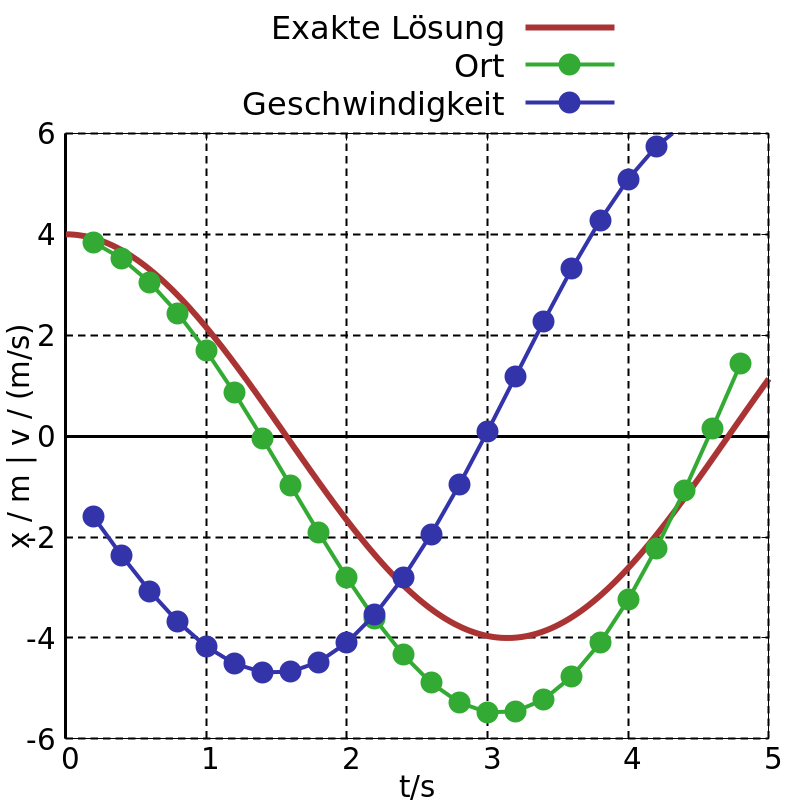
\includegraphics[width=0.65\textwidth]{./img/oscillation_dt_large}
    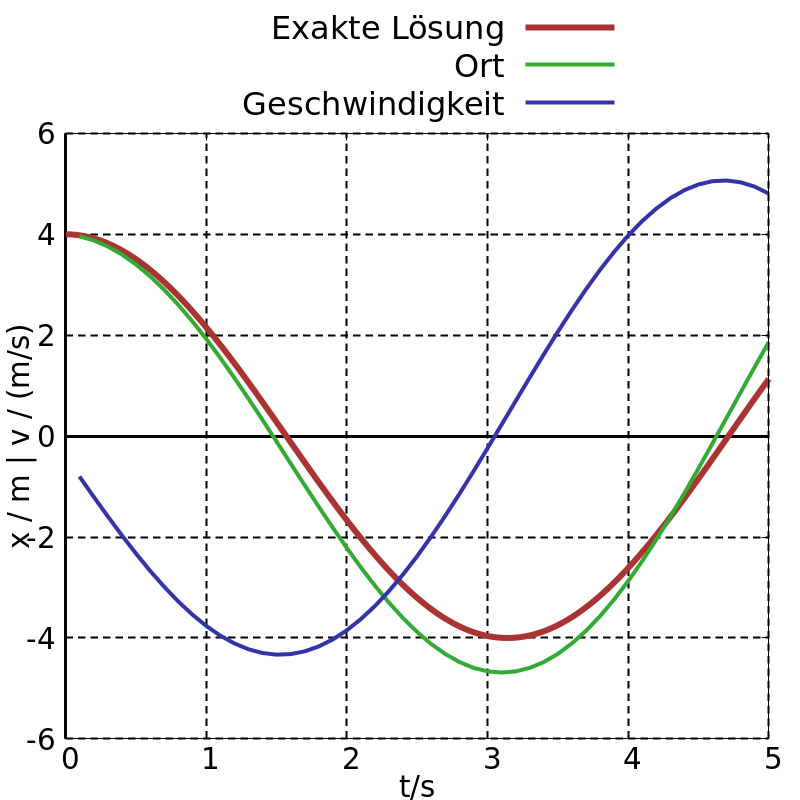
\includegraphics[width=0.48\textwidth]{./img/oscillation_dt_small}
    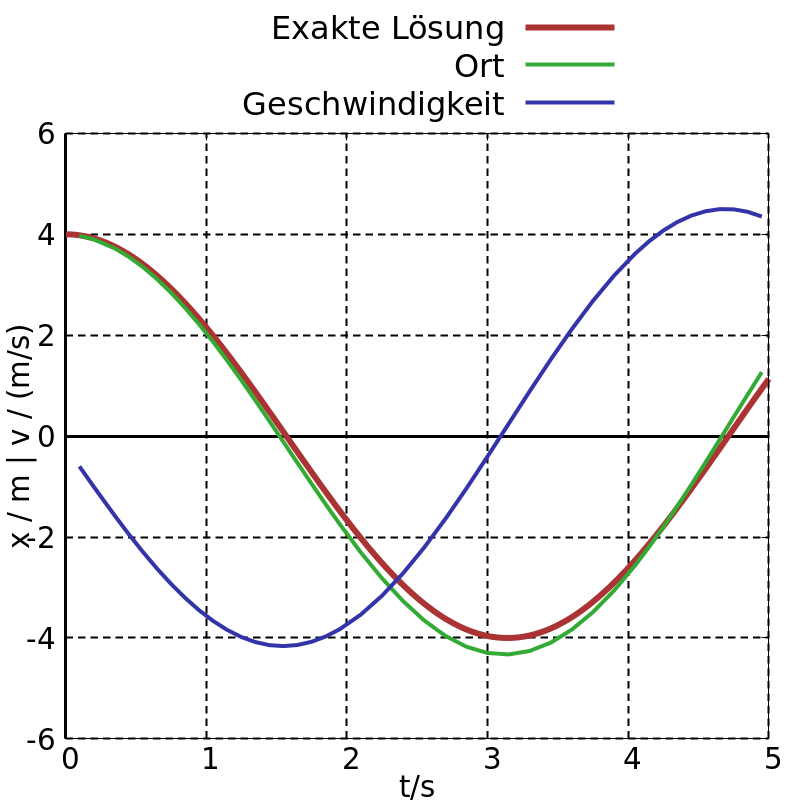
\includegraphics[width=0.48\textwidth]{./img/oscillation_dt_smallest}
    \caption[Nummerische Lösung der Schwingungsgleichung]{Nummerische Lösung der Schwingungsgleichung $y''-\frac{k}{m}y = 0$ für $k=1 \umss, m=1 \ukg$ und verschiedene Zeitschritt $\Delta t$. Oben: $\Delta t=0.2\us$. Unten links: $\Delta t=0.1\us$. Unten rechts: $\Delta t=0.05\us$.}
    \label{fig:DeqNumSolve}
\end{figure}

\section{Begriff der Differentialgleichung}

Zuerst müssen wir klären, was wir unter einer Differentialgleichung verstehen und was es bedeutet, eine Differentialgleichung zu lösen.

\begin{definition}{Differentialgleichung}{Deq}
    Eine Gleichung, welche eine Funktion sowie einer oder mehrere ihrer Ableitung enthält, nennt man \textbf{Differentialgleichung} (\textbf{DGL}).
\end{definition}

\begin{definition}{Ordnung einer DGL}{DeqOrder}
    Unter der \textbf{Ordnung $n$} einer DGL versteht man die höchste vorkommende Ableitung.
\end{definition}

So sind etwa folgende Gleichungen alle DGL:

\begin{itemize}
    \item $y' = y$ beziehungsweise $\dd{}{x} y = y$. Diese hat die Ordnung $1$, da $y'$ die höchste vorkommende Ableitung ist.
    \item $(y')^2 + 3 y' = \sin(y)$. Diese hat ebenfalls die Ordnung $1$.
    \item $y''+y'+4y=x^2$. Diese hat die Ordnung $2$, da $y''$ die höchste vorkommende Ableitung ist.
    \item $\pdd{f}{x} = \pdd{f}{y}$. Diese hat die Ordnung $1$, da nur erste partielle Ableitung nach $x$ und $y$ vorkommen.
\end{itemize}

Anmerkung zur Schreibweise: Um Schreibarbeit zu sparen, lässt man in oft das Argument der Funktion aus, also etwa $y'=y$ statt $y'(x) = y(x)$.

Im letzten Beispiel kamen partielle Ableitungen vor. Man unterscheidet allgemein zwischen DGL mit einstelligen Funktionen und DGL mit mehrstelligen Funktionen.

\begin{definition}{Ordinäre und partielle DGL}{OrdPartDGL}
    Eine DGL für eine einstellige Funktion nennt man \textbf{ordinäre DGL} (gewöhnliche DGL). Bei einer DGL mit einer zwei- oder mehrstelligen Funktionen spricht man von einer \textbf{partiellen DGL}.
\end{definition}

\begin{example}{Ordinäre und partielle DGL}{}
    \begin{itemize}
        \item $y''+2y=0$ ist eine gewöhnliche DGL.
        \item $\pdd{B_x}{x} + \pdd{B_y}{y} + \pdd{B_z}{z} = 0$ ist eine partielle DGL. Dabei ist $B$ das Magnetfeld. Diese DGL ist eine Teil der Maxwell-Gleichungen aus der Elektrodynamik und beschreibt die Tatsache, dass es keine magnetischen Monopole (Ladungen) gibt.
        \item $\pdd{u}{t} = k \cdot (\pddn{2}{u}{x} + \pddn{2}{u}{y} + \pddn{2}{u}{z})$ ist ebenfalls eine partielle DGL. Dabei ist $u$ die Temperatur an einem Punkt $(x,y,z)$ im Raum zu einem bestimmten Zeitpunkt $t$. Diese sogenannte Wärmeleitungsgleichung beschreibt, wie sich die Temperatur im Laufe der Zeit verändert. $k$ ist eine materialabhängige Konstante, welche ein Maß für die Temperaturleitfähigkeit ist.
    \end{itemize}
\end{example}

In dieser Vorlesung werden wir uns auf DGL mit einstelligen Funktionen beschränken.

\begin{definition}{Lösungen einer DGL}{DeqSol}
    Eine \textbf{Lösung} einer DGL $n$-ter Ordnung ist eine Funktion derart, dass die Gleichung für alle Argumente aus dem Definitionsbereich erfüllt ist. Die Menge aller Lösungen nenn man \textbf{allgemeine Lösung}, welche eine Kurvenschar mit $n$ willkürlichen wählbaren Parametern darstellt. Eine konkrete Lösungsfunktion aus dieser Schar entsteht durch eine konkrete Wahl der $n$ Parameter und wird \textbf{partikuläre Lösung} genannt. Eine Lösungsfunktion, welche nicht aus der allgemeinen Lösung durch Wahl durch eine bestimmte Belegung der Parameter entsteht, nennt man \textbf{singuläre Lösung}.
\end{definition}

\begin{example}{Probe für die Lösung einer DGL}{SolDeqCheck}
    Um zu überprüfen, ob eine vorgeschlagene Lösung tatsächlich eine DGL löst, können wir analog zu "normalen" Gleichungen eine Probe durchführen. Wir setzen die vorgeschlagene Lösung in die DGL ein und prüfen, ob sich eine wahre Aussage ergibt. Von der DGL $\tan(y) + y' = 0$  wird behauptet, dass $y(x) =  \asin\left(e^{C-x}\right)$ eine Lösung wäre. Um dies zu überprüfen, bilden wir zunächst die erste Ableitung $y'$. Mithilfe der Kettenregel \ref{stmt:ChainRule} und der Ableitung der Arkussinusfunktion aus Beispiel \ref{ex:CompDiffArcsin} erhalten wir:
    $$
        y' = \dd{}{x} \asin\left(e^{C-x}\right) = \frac{1}{\sqrt{1-\left(e^{C-x}\right)^2}} \cdot e^{C-x} \cdot (-1)
    $$
    Zudem benötigen wir noch $\tan(y)$. Es gilt $\tan(y) = \frac{\sin(y)}{\cos(y)}$ und damit folgt:
    \begin{alignat*}{1}
        \tan(y) &= \frac{\sin(\asin\left(e^{C-x}\right))}{\cos(\asin\left(e^{C-x}\right))} \\
                &= \frac{e^{C-x}}{\sqrt{1-\left(e^{C-x}\right)^2}}
    \end{alignat*}
    Durch Vergleich der Ausdrücke für $y'$ und $\tan(y)$ erkennen wir, dass diese sich nur im Vorzeichen unterscheiden. Daher gilt, wenn wir beide Ausdrücke in die DGL einsetzen $\tan(y) + y' = 0$. Somit haben wir gezeigt, dass $y(x) =  \asin\left(e^{C-x}\right)$ tatsächlich eine Lösung ist.
\end{example}

\begin{example}{Arten von Lösungen einer DGL}{DeqSolType}
    \begin{itemize}
        \item Die DGL $y'=y$ etwa beschreibt Funktionen, die identisch mit ihrer Ableitung sind. Eine solche Funktion kennen wir bereits: die Exponentialfunktion $y=e^x$. Setzen wir dieses $y$ in $y'=y$ ein, so erhalten wir $(e^x)'=e^x$. Das ist eine wahre Aussage, also ist $y=e^x$ eine \emph{partikuläre} Lösung der DGL. Gibt es noch mehrere Lösungen? Wir wissen, dass ein konstanter Vorfaktor in der Ableitung einfach mitgezogen wird. Also sind alle Funktionen der Form $y=C\cdot e^x$ mit beliebigen $C\in\R$ die allgemeine Lösung der DGL $y'y$. Eine weitere partikuläre Lösungen erhalten wir, in dem wir beispielsweise $C=-3$ setzen: $y(x) = -3 e^x$.
        \item Die DGL $y'^2 + y^2 = 1$ hat die allgemeine Lösung $y(x) = \pm \sin(C+x)$. Eine partikuläre Lösung ist beispielsweise $y(x) = \sin(3+x)$. Zudem ist aber auch $y(x) = \pm 1$ eine Lösung, was man durch Einsetzen in die DGL nachprüfen kann. Da diese beiden Lösungen nicht durch wahl von $C$ aus  $y(x) = \pm \sin(C+x)$ entstehen, handelt es sich um \emph{singuläre Lösungen}.
    \end{itemize}
\end{example}

Im obigen Beispiel \ref{ex:DeqSolType} haben wir gesehen, dass die allgemeine Lösung eine Funktionsgleichung mit einer frei wählbaren Konstante ist, also eine parametrisierte Kurvenschar darstellt. Für die meisten DGL wird das der Fall sein, die allgemeine Lösung enthält in der Regel eine oder mehrere Konstanten. Diese Konstanten entstehen unter Anderem durch die Integrationskonstante des unbestimmten Integrals. Daher ist es wichtig, diese nicht zu vergessen, da man sonst statt der allgemeinen Lösung nur eine partikuläre Lösung erhält.

Um nun eine Lösung einer DGL zu finden, gibt es gewissen Rechenverfahren, die wir später kennen lernen werden. Zuerst wollen wir uns aber mit einfachen DGL vertraut machen und uns anschauen, wie man diese graphisch lösen kann. Diese graphische Lösung stellt auch die Idee für nummerische Lösungsmethoden dar, die man anwenden kann, wenn sich eine DGL nicht mehr geschlossen lösen lässt.

\begin{definition}{Richtungsfeld einer DGL}{SlopeField}
    Eine DGL der Form $y'(x) = g(y,x)$, in der nur eine einstellige Funktion und deren erste Ableitung vorkommt, kann graphisch durch ein \textbf{Richtungsfeld} dargestellt werden. Das Richtungsfeld weist jedem zweidimensionalen Punkt $(x,y)$ einen \textbf{Richtungspfeil} in Richtung des Anstieg $y'$ und frei wählbaren Betrag zu. Ausgehend von einem Startpunkt lässt sich dann durch Folgen der Pfeile graphisch eine partikuläre Lösung ermitteln.
\end{definition}

\begin{example}{Ermittlung des Richtungsfelds}{CompSlopeField}
    Wir wollen graphisch die Lösung von $-x \cdot y'=y$ bestimmen. Um das Richtungsfeld zeichnen zu können, müssen wir sie zuerst in die Form $y'(x) = g(y,x)$ umformen -- also nach $y'$ umstellen. Für $x \ne 0$ gilt $y' = -y/x$. Das Richtungsfeld ergibt sich also, indem wir in einem zweidimensionalen Koordinatensystem an jedem Punkt $(x,y)$ einen Pfeil in Richtung des Anstieg einzeichnen. Wenn wir etwa $\Delta x$ Einheiten nach rechts gehen, müssen wir $y' \cdot \Delta x = -\frac{y}{x} \cdot \Delta x$ Einheiten nach oben gehen. Etwa für $Delta x = 1$ ergibt sich, dass der Richtungspfeil am Punkt $(x,y)$ lauten muss: $(1,-frac{y}{x})$. Zweckmäßigerweise normiert man alle Richtungspfeilen so, dass sie die gleiche Länge haben und sich gegenseitig nicht überlappen.
    Um die Arbeit beim Zeichnen des Richtungsfelds zu verringern, können wir uns noch überlegen, wo sich Linien gleichen Anstieg befinden. Damit $y'=const.$ gilt, muss der Quotient $y/x$ konstant sein, $y$ muss also ein Vielfaches von $x$ sind. Daher gilt, dass auf allen Geraden durch den Ursprung (etwa $y=2x$ oder $y=-5x$) die Richtungspfeile in die gleiche Richtung zeigen. Solche Linien gleichen Anstieg nennt man auch Isokline, von \emph{ísos} ("gleich") und \emph{inclination} ("Neigung").
\end{example}

\begin{figure}
    \centering
    \includegraphics[width=0.65\textwidth]{./gnuplot/example-slope-field}
    \caption[Richtungsfeld einer DGL]{Richtungsfeld der DGL $y'=-y/x$ und mögliche Anfangswerte der partikulären Lösungen}
    \label{fig:ExSlopField}
\end{figure}

In Abbildung \ref{fig:ExSlopField} ist solch ein Richtungsfeld dargestellt. Wir erkennen in dieser Abbildung auch noch etwa anderes. Um im Richtungsfeld eine partikuläre Lösungen einzuzeichnen, müssen wir den Pfeilen folgen. Doch dazu benötigen wir einen Startpunkt. Je nachdem, welchen Startpunkt wir wählen, erhalten wir eine andere Kurve. Oder anders ausgedrückt: das Richtungsfeld zeigt alle möglichen Lösungen (\emph{allgemeine Lösung}), eine konkrete Lösung (\emph{partikuläre Lösung}) wird dadurch ausgewählt, dass wir einen Punkt $(x,y)$ vorgeben, durch den die Kurve verlaufen soll.

\begin{definition}{Anfangs- und Randbedingungen}{InitBoundCond}
    Um eine partikuläre Lösung einer DGL $n$-ter Ordnung eindeutig zu bestimmen, werden neben der DGL noch zusätzliche Einschränkungen (im allgemeinen $n$ Stück) an die Lösungsfunktion benötigt. Dabei gibt es zwei wesentliche Arten von Bedingungen:
    \begin{itemize}
        \item Bei einem \textbf{Anfangswertproblem} sind \textbf{Anfangsbedingungen} gegeben, also der Wert der Funktion oder ihrer Ableitungen an einer Stelle.
        \item Bei einem \textbf{Randwertproblem} sind \textbf{Randbedingungen} gegeben, also der Wert der Funktion oder ihrer Ableitung am Rande eines betrachteten Gebiets.
    \end{itemize}
\end{definition}

Ein physikalisches Beispiel für ein Anfangswertproblem ist etwa der freie Fall, wenn Anfangsort x und Anfangsgeschwindigkeit $\dot{x} = \dd{x}{t}$ zum Zeitpunkt $t_0$ vorgegeben ist. Randwertprobleme treten meist bei partiellen Differentialgleichungen auf, beispielsweise kann man in der Elektrostatik das elektrische Potential $\varphi$ am Rand eines geerdeten Leiters vorgeben. Ein weiteres Beispiel für ein Randwertproblem ist Seil, welches an zwei Enden eingespannt ist. Damit ist die Position des Seils am Rand fest vorgeben, die Bewegung des Seils zwischen beiden Enden wird dann durch die Schwingungsgleichung beschrieben.

\begin{example}{Lösen einer DGL mit Anfangsbedingung}{SolDeqInitCond}
    Die DGL der ungestörten harmonischen Schwingung lautet $y''+y=0$. Die allgemeine Lösung dieser DGL (wie wir später noch berechnen werden), lautet $y(x) = C_1 \sin(x) + C_2 \cos(x)$. Als Anfangsbedingung ist gegeben $y(\pi/4)=2$ (Auslenkung des Pendels zum Zeitpunkt $\pi/4$) und $y'(\pi/4)=-2$ (Geschwindigkeit des Pendels zum Zeitpunkt $\pi/4$). Wir setzen beide Bedingungen in die allgemeine Lösung ein und bestimmen daraus die noch offenen konstanten $C_1$ und $C_2$. Dazu benötigen wir die Ableitung $y'(x) = C_1\cos(x) - C_2\sin(x)$. Wir erhalten:
    \begin{alignat*}{1}
        y(\pi/4) &= C_1 \sin(\pi/4) + C_2\cos(\pi/4) = \frac{\sqrt{2}}{2} (C_1+C_2) = 2 \\
        y'(\pi/4) &= C_1 \cos(\pi/4) - C_2\sin(\pi/4) = \frac{\sqrt{2}}{2} (C_1-C_2) = -2
    \end{alignat*}
    Damit erhalten wir das lineare Gleichungssystem
    $$
        C_1+C_2=2\sqrt{2}
        C_1-C_2=-2\sqrt{2}
    $$
    Daraus ergibt sich $C_1=0$ und $C_2=2\sqrt{2}$ und die partikuläre für die gegebene Anfangsbedingung lautet:
    $$
        y_P(x) = 2\sqrt{2}\cos(x)
    $$
\end{example}

\section{Homogenität und Linearität}

Zwei wichtige Eigenschaften von DGL sind die sogenannten Homogenität und Linearität. Wir werden sehen, dass speziell lineare DGL einfacher lösbar sind als nichtlineare DGL. Die Navier-Stokes-Gleichung beschreibt wie bereits erwähnt Phänomene der Fluiddynamik. Es handelt es sich dabei um eine partielle und nichtlineare DGL. Aufgrund ihrer Nichtlinearität ist diese bisher noch nicht vollständig gelöst. Eines der sieben Millennium-Problem des \href{http://www.claymath.org/millennium-problems}{Clay Mathematics Institute} betrifft diese DGL:

\begin{quotation}
    \textbf{Navier–Stokes Equation}. This is the equation which governs the flow of fluids such as water and air. However, there is no proof for the most basic questions one can ask: do solutions exist, and are they unique? Why ask for a proof? Because a proof gives not only certitude, but also understanding.
\end{quotation}

Um die eben erwähnten Begriffe genau zu definieren, benötigen wir zunächst erstmal die kanonische Darstellungsform einer gewöhnlichen DGL. Kanonisch leitet sich ab vom Lateinischen \emph{canon} (\emph{Norm}, \emph{Regel}) und meint in der Mathematik eine konkrete Darstellungsweise aus vielen möglichen Darstellungsweisen.

\begin{definition}{Formen der Gleichung einer DGL}{DeqForms}
    Die Gleichung einer DGL $n$-ter Ordnung kann in verschiedene Formen umgestellt werden. Eine konkrete Form der Gleichung einer DGL heißt
    \begin{itemize}
        \item \textbf{explizit}, wenn die höchste Ableitung $y^{(n)}$ alleine auf der linken oder rechten Seite der Gleichung steht.
        \item \textbf{implizit}, wenn sie nicht explizit ist.
        \item \textbf{kanonisch}, wenn alle Glieder auf einer Seite der Gleichung stehen, also sich schreiben lässt als $\Phi(y,y',y'',y''',\dots,y^{(n)},x) = 0$
    \end{itemize}
\end{definition}

\begin{example}{DGL in expliziter und impliziter Form}{ExExplImplDeq}
    \begin{itemize}
        \item $\sin(y'+x^2) = y''$ ist explizit, da $y''$ alleine auf der rechten Seite steht.
        \item $\sin(y''+x^2) = y'$ ist implizit, da $y''$ innerhalb des Terms auf der linken Seite vorkommt.
        \item $\sin(y''+x^2) = y''$ ist implizit, da $y''$ auf beiden Seiten der Gleichung vorkommt.
        \item $y''+x=0$ ist implizit, umgeformt zu $y''=-x$ erhält man die explizite Form.
    \end{itemize}
\end{example}

\begin{example}{Kanonische Form einer DGL}{ExCanonDeq}
    \begin{itemize}
        \item Die DGL $y''+2y'-y=2x$ lässt sich umstellen zu $-y+2y'+y''-2x=0$. Das ist eine kanonische Form, sich lässt sich schreiben als $\Phi(y,y',y'',x)=-y+2y'+y''-2x=0$.
        \item Im Allgemeinen lässt sich jede DGL $\dots = \dots$ auf kanonische Form bringen, indem man durch Subtraktion die rechte Seite auf die linke Seite bringt.
    \end{itemize}
\end{example}

Mithilfe der Notation $\Phi(y,y',y'',y''',\dots,y^{(n)},x) = 0$, also dass wir die DGL als einen Term auffassen können, in dem das Argument, die Funktion und ihre Ableitungen vorkommen, können wir nun die nächste Eigenschaft einer DGL formulieren.

\begin{definition}{Homogenität}{HomogenousDeq}
    Eine DGL $n$-ter Ordnung $\Phi(y,y',y'',y''',\dots,y^{(n)},x) = 0$ heißt \textbf{homogen}, falls sie eine homogene Gleichung in der gesuchten Funktion $y$ und ihren Ableitung ist, das heißt, falls es ein $\alpha\in¸N_0$ gibt, sodass gilt:
    $$
        \forall t: \Phi(ty,ty',ty'',ty''',\dots,ty^{(n)},x) = t^\alpha \cdot \Phi(y,y',y'',y''',\dots,y^{(n)},x)
    $$
    $\alpha$ heißt dann \textbf{Grad der Homogenität}. Andernfalls heißt die DGL \textbf{inhomogen}.
\end{definition}

Anders formuliert bedeutet die Gleichung in obiger Definition, dass wir, wenn wir alle $y$ mit einer Konstante multiplizieren, diese Konstante aus der gesamten Gleichung ausklammern können. Der Begriff der Homogenität ("Gleichförmigkeit") geht auf die Definition sogenannten \emph{homogener Funktionen} zurück. Eine Funktion heißt beispielsweise homogen, falls sich ihr Funktionswert verdoppelt, wenn man das Argument verdoppelt -- der Funktionswert also gleichmäßig mit dem Argument skaliert. Lineare Gleichungen der Form $y=mx$ sind homogen (vom Grad 1). Ein anderes Beispiel für homogene Funktionen sind Parabeln $y=ax^2$. Wenn wir das Argument verdoppeln, vervierfacht sich der Funktionswert. Allgemeiner können wir sagen, dass wenn wir das Argument mit $t$ multiplizieren (skalieren), der Funktionswert mit $t^2$ multipliziert wird: $f(tx)=t^2f(x)$. Noch allgemeiner heißt eine Funktion $f$ homogen vom Grad $\alpha$, wenn $f(tx) = t^\alpha f(x)$ gilt. Bei einer homogenen Funktionen steht also die Skalierung entlang der Abszisse (x-Achse) in einem Zusammenhang mit der Skalierung entlang der Ordinate (y-Achse). Wenn wir jetzt nochmal an die Definition für homogene DGL zurückdenken, so stellen wir fest, dass sie der Definition einer homogenen Funktion ähnelt, nur mit dem Unterschied, dass wir jetzt mehrere Argumente gleichzeitig skalieren.

\begin{example}{Überprüfung der Homogenität}{ExHomoDeq}
    \begin{itemize}
        \item $y''+xy=0$ ist homogen, denn wenn wir alle $y$ mit $t$ multiplizieren, erhalten wir $ty''+xty$, und hier können wir $t$ vollständig aus allen Summanden ausklammern: $t^1 \cdot (y''+xy)$. Der Grad der Homogenität ist wegen $t^1$ gleich 1.
        \item $y''+xy-3=0$ ist inhomogen. Wenn wir alle $y$ mit $t$ multiplizieren, erhalten wir $ty''+xty-3$. Da im letzten Summanden $-3$ kein $t$ vorkommt, können wir es nicht vollständig ausklammern. Anders betrachtet ist es uns also nicht möglich, in der Gleichung $ty''+xty-3 = t^n \cdot (y''+xy-3)$ einen Wert für $n$ zu finden, sodass daraus eine wahre Aussage wird.
        \item $y''+xy-3x=0$ ist inhomogen. Wenn wir alle $y$ mit $t$ multiplizieren, erhalten wir $ty''+xty-3x$. Da im letzten Summanden $-3x$ kein $t$ vorkommt, können wir es nicht vollständig ausklammern.
        \item $y''+xy^2=0$ ist inhomogen. Nach Multiplikation mit $t$ erhalten wir $ty''+xt^2y^2$. Im ersten Summanden kommt $t$ zur Potenz $1$ vor, im zweiten Summanden zur Potenz $2$. Wir können daher weder $t$ noch $t^2$ auf beiden Seiten ausklammern.
        \item $(y')^2+y^2=0$ ist homogen vom Grad $2$. Wir setzen an $(ty')^2+(ty)^2=t^2\cdot\left[(y')^2+y^2\right]$. Da $t^2$ in beiden Summanden vorkommt, konnten wir es vollständig ausklammern. Wegen $t^2$ ist der Grad der Homogenität $2$.
        \item $\sin(x)y'''+x^2y=0$ ist homogen vom Grad $1$, denn $\sin(x)ty'''+x^2 t y = t^1 \cdot \left(\sin(x)y''+x^2y\right)$.
        \item $\frac{y'}{y}+x=0$ ist homogen vom Grad $0$, denn $\frac{ty'}{ty}+x = t^0 \cdot \left(\frac{y'}{y}+x\right)$.
   \end{itemize}
\end{example}

Anhand der obigen Beispiel können wir einige Beobachtungen machen, welche uns das Überprüfen der Homogenität erleichtern. Kommt in der Funktionsgleichung ein Summand (ungleich 0) vor, in dem kein $y$ oder eine Ableitung von $y$ steht, ist die DGL in der Regeln inhomogen. Die einzige Ausnahme tritt auf, wenn die restlichen Terme Quotienten von $y$ sind, sodass sich ein Grad der Homogenität $0$ ergibt. Im folgenden werden wir hauptsächlich DGL betrachten, wo der Grad der Homogenität $1$ ist, daher ist diese Faustregel sehr hilfreich.  Weiterhin stellen wir noch fest, dass eine homogene DGL mit Grad der Homogenität $1$ vorliegt, wenn $y$ in allen weiteren Summanden ohne weitere Rechenoperation (Quadrieren, Sinusbildung, \dots) vorkommt und höchstens noch einen Vorfaktor hat. Solche Arten von DGL nennt man lineare homogene DGL, welche wir in einem der nächsten Abschnitte noch genauer betrachten werden.

Des Weiteren können wir noch eine Feststellung machen, wenn wir uns die ersten drei Beispiele noch einmal genauer anschauen: $y''+xy=0$ ist homogen, $y''+xy-3=0$ bzw. $y''+xy-3x=0$ jedoch nicht. Der Unterschied besteht im Summanden $-3$ beziehungsweise $-3x$. Während die letzten beiden DGL zwar nicht homogen sind, können wir sie zerlegen in eine Summe aus einer homogenen DGL ($y''+xy=0$) und einem Inhomogenitäts-Term ($-3$ beziehungsweise $-3x$).

\begin{definition}{Homogener und inhomogener Anteil}{HomInhomPart}
    Einige inhomogene DGL $n$-ter Ordnung lassen sich zerlegen in einen homogenen und einen inhomogenen Anteil:
    $$
        \Phi(y,y',y'',y''',\dots,y^{(n)},x) = 0 = \underbrace{H(y,y',y'',y''',\dots,y^{(n)},x)}_{Homogener Anteil} + \underbrace{F(x)}_{\text{Inhomogenität}}
    $$
    Ist dies möglich, so heißt $H$ der \textbf{inhomogene Anteil} der DGL und $H(y,y',y'',y''',\dots,y^{(n)},x) = 0$ die zur DGL \textbf{zugehörige homogene DGL}. Weiterhin heißt $F$ die \textbf{Inhomogenität} der DGL.
\end{definition}

Kleiner Hinweis zur Notation: Oft bringt man den inhomogenen Anteil $F(x)$ auch auf die rechte Seite der Gleichung und nennt dann $-F(x)$ die Inhomogenität:

$$
    H(y,y',y'',y''',\dots,y^{(n)},x) = \underbrace{-F(x)}_{\text{Inhomogenität}}
$$

\begin{example}{Zerlegung einer inhomogenen DGL}{ExHomInhomPart}
    \begin{itemize}
        \item Die zu $y''+xy=3x$ zugehörige homogene DGL lautet $y''+xy=0$, die Inhomogenität ist $3x$.
        \item Die DGL $y''+y = \sin(2 \pi x)$ beschreibt physikalisch ein schwingendes Pendel. Die zugehörige homogene DGL $y''y=0$ stellt eine freischwingendes Pendel dar, die Inhomogenität $\sin(2 \pi x)$ ergibt sich, wenn man das Pendel etwa mit einem Motor sinusförmig mit der Frequenz $1$ antreibt (erzwungene Schwingung).
        \item Die DLG $y''+xy=0$ ist bereits homogen und stellt damit selbst ihre zugehörige homogene DGL dar, die Inhomogenität ist $0$.
        \item Die DGL $\sin(y)=x$ ist inhomogen und lässt sich nicht in einen homogenen und inhomogenen Anteil zerlegen.
    \end{itemize}
\end{example}

Wie erwähnt sind lineare DGL von besonderem Interesse, nicht nur, da sie sich leicht lösen lassen, sondern auch zur Modellierung vieler Phänomene verwendet werden können. Die Linearität ist eine spezielle Form der Homogenität:

\begin{definition}{Lineare DGL}{LinDeq}
    Eine DGL $n$-ter Ordnung nennt man \textbf{linear}, wenn sie einen homogenen Anteil $H(y,y',y'',y''',\dots,y^{(n)},x)$ besitzt und dieser den Grad der Homogenität $1$ besitzt. Andernfalls heißt sie \textbf{nichtlinear}.
\end{definition}

Um eine Homogenität vom Grad $1$ zu erreichen, dürfen die gesuchte Funktion $y$ und alle ihre Ableitungen nur als lineare Summanden mit Vorfaktor (Koeffizient) in der DGL vorkommen. Wir man sich überlegen kann, ist die allgemeine Form solcher linearen DGL $n$-ter Ordnung:

$$
    \sum\limits_{i=0}^{n} a_i(x) y^{(i)}(x) = F(x)
$$

Wobei die Koeffizienten $a_i(x)$ beliebige, nur von $x$ abhängige Funktionen sind und $F(x)$ die Inhomogenität ist. Einige Beispiele für solche linearen DGL sind etwa:

\begin{itemize}
    \item $y'=0$
    \item $y'''-7y''+2y''+y'-5y=\sin(x)\cdot e^x$
    \item $\sin(x)x^2y'''+4e^x y = x$
\end{itemize}

Für nichtlineare DGL sind einige Beispiel etwa:

\begin{itemize}
    \item $\sin(y')=y$
    \item $\frac{y''}{y'} = y^2$
    \item $(y')^2+y=0$
\end{itemize}

\section{Direkte Integration}

In den verbleibenden Abschnitten wollen wir uns noch einige übliche Lösungsmethoden für DGL anschauen. Aufgrund der Knappheit der Zeit müssen wir uns dabei auf einige grundlegende Verfahren beschränken. Auf die Theorie der Lösung von Differentialgleichungssystem mit mehr als einer Funktion $y$ können wir hier gar nicht eingehen.

Die vermutlich einfachste Lösungsmethode einer DGL besteht in ihrer direkten Integration. Falls die DGL $n$-ter Ordnung in der Form $y^{(n)} = f(x)$ vorliegt, so müssen wir nur $n$-mal das unbestimmte Integral bilden und erhalten so die allgemeine Lösung der DGL mit $n$ Konstanten.

\begin{example}{Freier Fall}{FreeFall}
    Das Newtonsche Grundgesetz lautet $\ddot{x} = \frac{1}{m}\cdot F(x,t)$. Dabei ist $\ddot{x} = \ddn{2}{x}{t}$ die zweite Ableitung des Ortes eines Körpers $x$ nach der Zeit $t$, $F$ die auf den Körper wirkende Kraft und $m$ seine Masse. Durch Lösen dieser DGL erhält man die Bahnkurve des Körpers. Für einen frei fallenden Körper nahe der Erdoberfläche gilt $F(x,t)=m \cdot g$ mit der Fallbeschleunigung $g\approx 9.8\umss$, falls die x-Achse in Richtung Erdboden zeigt. Damit lautet die Bewegungsgleichung für einen frei fallenden Körper $\ddot{x} = g$. Diese DGL können wir durch zweifache direkte Integration lösen. Die erste Integration liefert:
    $$
        v(t) = \dot{x}(t) = \int g \diff{x} = gt +v_0
    $$
    Dabei ist $v$ die Geschwindigkeit, welche per Definition die erste Ableitung des Ortes nach der Zeit ist. Die Integrationskonstante $v_0$ hat eine physikalische Bedeutung, nämlich die Anfangsgeschwindigkeit des Körpers zum Zeitpunkt $t=0$. Erneute Integration liefert:
    $$
        x(t) = \int gt + v_0 \diff{x} = \frac{1}{2} g t^2 + v_0 t + s_0
    $$
    Dabei ist $s_0$ der Anfangsort des Körpers zum Zeitpunkt $t=0$. Die DGL hat die Ordnung $2$, insgesamt haben wir wie erwartet die $2$ Integrationskonstanten $v_0$ und $s_0$ gewonnen. Durch Lösen der Bewegungsgleichung für den freien Fall haben wir somit die bekannte Formel für den freien Fall erhalten.
\end{example}

\section{Trennung der Variablen}

Diese Lösungsstrategie hilft bei DGL 1. Ordnung, die sich als Produkt zweier Terme schreiben lassen, wobei ein Term nur von der unabhängigen Variable $x$ und der andere Term nur von dem Funktionswert $y$ abhängt. Wir betrachten also DGL der Form

$$
   y'(x) = f(x) g(y)
$$

Wobei $f$ und $g$ beliebige differenzierbare und integrierbare Funktionen sind. Um diese DGL zu lösen, formen wir um

$$
    \frac{1}{g(y)} y'(x) =  f(x)
$$

und integrieren beide Seiten nach $x$:

\begin{equation}
    \int \frac{1}{g(y(x))} y'(x) \diff{x} =  \int f(x) \diff{x} \label{eq:SepVarProof1}
\end{equation}

Die linke Seite der Gleichung können wir vereinfachen, indem wir die Regel für die Integration durch Substitution (siehe Aussage \ref{stmt:IntSubst}) anwenden. Diese Regel lautet mit $f(u) = \frac{1}{g(u)}$:

$$
    \int \frac{1}{g(u)} \diff{u} = \int \frac{1}{g(u(t)} u'(t) \diff{t}
$$

Mit der Umbenennung $t \to x$ und $u \ to y$ wird daraus:

\begin{equation}
    \int \frac{1}{g(y)} \diff{y} = \int \frac{1}{g(y(x)} y'(x) \diff{x} \label{eq:SepVarProof2}
\end{equation}

Aus \ref{eq:SepVarProof1} und \ref{eq:SepVarProof2} folgt damit das Verfahren der Trennung der Variablen:

\begin{statement}{Trennung der Variablen}{SeparationOfVariables}
    Eine gewöhnliche DGL 1. Ordnung, welche sich in der Form $y' = f(x) \cdot g(y)$ schreiben lässt, besitzt eine allgemeine Lösung $y(x)$, welche durch folgende implizite Funktionsgleichung gegeben ist:
    $$
        \int \frac{1}{g(y)} \diff{y} = \int f(x) \diff{x} + C
    $$
    Dabei ist $C \in \R$ eine freie Konstante für die allgemeine Lösung.
\end{statement}

Mithilfe der Leibniz-Notation können wir dieses Verfahren auch wie folgt schreiben:

\begin{alignat*}{1}
    y'        &= f(x) g(y) \\
    \dd{y}{x} &= f(x) g(y) \\
    \frac{\diff(y)}{g(y)}      &= f(x) \diff{x} \\
    \int \frac{\diff(y)}{g(y)} &= \int f(x) \diff{x}
\end{alignat*}

Hier sehen wir auch noch einmal, warum sich dieses Verfahren \emph{Trennung der Variablen} nennt. Indem wir alle Terme mit $x$ und alle Terme mit $y$ auf jeweils die linke und die rechte Seite der Gleichung bringen, trennen wir Variablen $x$ und $y$. Wenn wir dies geschafft haben, können wir beide Seiten integrieren, um die Lösung der DGL zu erhalten.

Es sei noch angemerkt, dass dieses Verfahren zwei Probleme hat. Während wir zwar eine Lösung der DGL gefunden haben, kommen in dieser Lösung noch unbestimmte Integrale vor. Wenn wir diese Integrale nicht lösen können, erhalten wir auch keine Lösung. Dies ist ein allgemeines Problem vieler Lösungsverfahren, welche es oft in der Lösungsformel erfordern, dass man Integrale lösen kann. Im Vergleich zum Differenzieren passiert es beim Integrieren häufig, dass wir keine geschlossene Formel finden können, selbst wenn der Integrand "einfach" aussieht. In diesem Fall kann man über nummerische Lösungsverfahren versuchen, eine Näherungslösung zu erhalten. Das zweite Problem an der Trennung der Variablen ist, dass es die gesuchte Lösungsfunktion nur in impliziter Form angibt. Selbst wenn wir die Integrale lösen können, müssen wir im Anschluss noch die Gleichung nach $y$ umstellen, was im Allgemeinen nicht immer möglich ist.

\begin{example}{Anwendung der Trennung der Variablen}{SepVar}
    Die DGL $y'=\frac{y}{x}$ ist von der Form $y' = f(x) \cdot g(y)$, wobei $f(x)=\frac{1}{x}$ und $g(y)=y$ ist. Mit der Leibniz-Notation erhalten wir aus $\dd{y}{x} = \frac{y}{x}$ durch Umstellen:
    $$
        \int \frac{\diff{y}}{y} = \int \frac{\diff{x}}{x}
    $$
    Die Integrale können wir lösen und erhalten:
    $$
        \ln(|y|) = \ln(|x|) + C
    $$
    Um diese implizite Funktionsgleichung für $y$ aufzulösen, wenden wir die Exponentialfunktion an:
    \begin{alignat}{1}
        e^{\ln(|y|)} &= e{\ln(|x|) + C} \\
        |y|          &= e^C |x| \\
        y            &= \pm e^C |x|
    \end{alignat}
    Während $e^C$ nur positive Werte annehmen kann, sind durch den Betrag für $\pm e^C$ sowohl positive als auch negative Werte möglich. Durch Einsetzen in die DGL bestätigen wir, dass $y(x) =0$ ebenfalls eine Lösung ist. Wir können daher $\pm e^C$ durch eine Konstante $C\in\R$ ersetzen und erhalten die allgemeine Lösung:
    $$
        y(x) = C |x|
    $$
    Die Menge aller Lösungen wird daher durch die Menge aller Geraden gegeben, die durch den Koordinatenursprung laufen.
\end{example}

Man beachte auch den Unterschied zwischen den DGL aus Beispiel \ref{ex:CompSlopeField} ($y'=-y/x$) und \ref{ex:SepVar} ($y'=y/x$). Obwohl diese sich nur in einem Vorzeichen unterscheiden, haben sich ganz verschiedene Lösungen, Hyperbeln beziehungsweise Geraden.

\begin{example}{Umgebremste Vermehrung einer Population}{ExpModel}
    Die ungebremste Vermehrung einer Population, etwa von Wildtieren, Seerosen, Bakterien oder Viren, findet statt, wenn ausreichend Ressourcen zur Verfügung stehen und die Vermehrung nicht gebremst wird. Mit $N(t)$ bezeichnen wir die Größe der Population in Abhängigkeit der Zeit $t$. Die zeitliche Ableitung $\dd{N}{t} = \dot{N}(t)$ ist dann ein Maß für die Änderung der Anzahl pro Zeiteinheit. Um ein Modell für das Wachstum der Population zu erhalten, überlegen wir uns, dass dieser Zuwachs direkt proportional ist zur Größe der Population: Wenn etwa 10 Rentieren in einem Jahr 20 junge Rentiere gebären, dann werden bei einer vierfachen Ausgangsgröße von 40 Rentieren auch viermal so viele Jungtiere (80) geboren. Unser Modell lautet damit:
    $$
        N'(t) \propto N(t)
    $$
    Die Proportionalitätskonstante bestimmt, wie schnell sich die Population vermehrt und wird beeinflusst etwa durch den Zyklus, in dem Wildtiere gebären, die Seerosen sich vermehren oder die Inkubationszeit. Bezeichnen wir die Proportionalitätskonstante mit $\alpha$, erhalten wir die DGL für das \textbf{exponentielle Wachstum}:
    $$
        N' = \alpha N
    $$
    Diese DGL kann mittels der Trennung der Variablen gelöst werden:
    \begin{alignat*}{1}
        \dd{N}{t}               &= \alpha N \\
        \int \frac{\diff{N}}{N} &= \int \alpha t \\
        \ln(|N|)                &= \alpha t + C \\
        N(t)                    &= C \cdot e^{\alpha t}
    \end{alignat*}
\end{example}

\begin{example}{Gebremste Vermehrung}{LogGrowthModel}
    Im vorigen Beispiel sind wir davon ausgegangen, dass die Population sich ungebremst vermehren konnte. Dies ist in der Realität meistens natürlich nicht der Fall, da Ressourcen und Energie immer begrenzt sind. Beispielsweise ist bei Wildtieren ein begrenzender Faktor die Verfügbarkeit von Nahrung, bei Seerosen die Größe des Teichs oder bei Viren die Verfügbarkeit von Wirten sowie deren Immunität. Um diesen Sachverhalt zu modellieren, gehen wir davon aus, dass es eine bestimmte Obergrenze für die Population gibt und nennen diese $K$. Je näher die Population an diese Obergrenze kommt, desto knapper werden die Ressourcen und desto langsamer findet die Vermehrung statt. Als einfachste Näherung nehmen wir an, dass die Zuwachsrate proportional ist zur Differenz $K-N$ (für $K=N$ ist sie $0$, sodass die Obergrenze nicht überschritten wird). Dies ist unser Modell für die Knappheitsphase, wo die Populationsgröße nahe der Obergrenze liegt. Falls die Größe aber weit weg von der Obergrenze ist, befinden wir uns wie im vorigen Beispiel in der Wachstumsphase. Hier modellieren wir den Zuwachs so, dass er proportional zur Populationsgröße ist. Um nun ein Gesamtmodel zu erhalten, multiplizieren wir beide Zuwachsraten und erhalten die DGL für das \textbf{logistische Wachstum}:
    $$
        N' = \alpha N (K-N)
    $$
    Diese DGL beschreibt ein gebremstes Wachstum und hat die allgemeine Lösung, welche man durch Trennung der Variablen findet:
    $$
        N(t) = \frac{Ke^{K \alpha (t - C)}}{e^{K \alpha (t  - C)} \pm 1}
    $$
    Durch die freie Konstante $C$ wird die Lösungsfunktion entlang der Abszisse verschoben, die Konstante beschreibt den Zeitpunkt, an dem der Wechsel zwischen der ungebremsten, exponentiellen Phase und der gebremsten Phase stattfindet. Im Nenner ist sowohl $+1$ als auch $-1$ möglich, dabei beschreibt der Fall $+1$ das hier betrachtete logistische Wachstum, der Fall $-1$ ergibt sich, wenn der die anfängliche Populationsgröße über der Obergrenze $K$ liegt und ist damit keine realistische Lösung. In Abbildung \ref{fig:ExSlopeFieldLogGrowth} sind das Richtungsfeld und einiger Lösungen dargestellt.
\end{example}

\begin{figure}
    \centering
    \includegraphics[width=0.75\textwidth]{./gnuplot/logistic-growth-slope-field}
    \caption[Richtungsfeld der logistischen DGL]{Richtungsfeld der DGL für den logistischen Wachstum mit $\alpha=0.5$ und $K=4$}
    \label{fig:ExSlopeFieldLogGrowth}
\end{figure}

\section{Variation der Konstanten}

Oft ist es bei der Lösung von DGL, dass man aufgrund der Erfahrung oder der Form einer DGL einen Ansatz macht, den noch freie Parameter oder Funktionen enthält, und dann durch Einsetzen in die DGL versucht, diese zu bestimmen. Gelingt dies, hat man eine Lösung der DGL gefunden. Ein solches Verfahren ist die Variation der Konstanten, welche beim Lösen einer inhomogenen DGL hilft. Man beginnt mit der allgemeinen Lösung der zugehörigen homogenen DGL, welche $n$ freie Konstanten $C_i$ enthält und tut dann so, als ob diese Konstanten nicht konstant wären, sondern ebenfalls Funktionen $C_i(x)$ des Arguments $x$. Diesen Ansatz setzt man dann in die inhomogene DGL ein und versucht die $C_i(x)$ so zu bestimmen, dass die DGL erfüllt ist.

Im Folgenden wollen wir inhomogene DGL 1. Ordnung der folgenden Form betrachten:

$$
    y'+P(x)y=Q(x)
$$

Dabei sind $P$ und $Q$ beliebige differenzierbare Funktionen. Die homogene DGL $y'+P(x)y=0$ lösen wir durch Trennung der Variablen:

\begin{alignat*}{1}
    \dd{y}{x}               &= -P(x) y \\
    \int \frac{\diff{y}}{y} &= -P(x) \diff{x} \\
    y(x)                    &= C \cdot e^{\int -P(x) \diff{x}}
\end{alignat*}

Für die weitere Betrachtung nutzen wir die Abkürzung $\hat{P}$ für die Stammfunktion von $P$.

Um nun die inhomogene DGL $y'+P(x)y=Q(x)$ zu lösen, machen wir nach dem Prinzip der Variation der Konstanten den Ansatz:

$$
    y(x) = C(x) \cdot e^{-\hat{P}(x)}
$$

Die Funktion $C(x)$ müssen wir so bestimmen, dass die DGL erfüllt ist. Dazu leiten wir den Ansatz für $y$ einmal ab und setzen ihn in die DGL ein:

\begin{alignat*}{1}
    y' &= C' e^{-\hat{P}} - C \hat{P}' e^{-\hat{P}} \\
       &= C' e^{-\hat{P}} - C P e^{-\hat{P}}
\end{alignat*}

Nun können wir den Ansatz $y$ und dessen Ableitung $y'$ in die DGL einsetzen:

\begin{alignat*}{1}
    y'+Py                                                 &= Q \\
    C' e^{-\hat{P}} \underbrace{- C P e^{-\hat{P}} + P C e^{-\hat{P}}}_{=0} &= Q \\
    C' e^{-\hat{P}} &= Q \\
\end{alignat*}

Damit haben wir einen Ausdruck für $C'(x)$ gefunden. Wir stellen nach $C'$ um und integrieren einmal, um $C$ zu erhalten:

\begin{alignat*}{1}
    C' &= Q e^{\hat{P}} \\
    C  &= \int Q e^{\hat{P}} \diff{x} + C_1
\end{alignat*}

Dabei ist $C_1 \in \R$ eine beliebige Konstante. Wir setzen nun das so gewonnene $C$ in unseren Ansatz ein und erhalten die allgemeine Lösung der DGL.

\begin{statement}{Separierbare inhomogene DGL 1. Ordnung}{SepInhDeqOrd1}
    Die allgemeine Lösung der inhomogenen DGL 1. Ordnung $y'+P(x)y=Q(x)$ lautet
    $$
        y(x) =  e^{-\int P(x) \diff{x}} \int Q(x) e^{\int P(x) \diff{x}} \diff{x}   + C e^{-\int P(x) \diff{x}}
    $$
\end{statement}

Diese Formel lässt sich schwer auswendig lernen. Für die praktische Berechnung ist es daher oft besser, sich nicht die fertige Formel zu merken, sonder das Vorgehen:

\begin{itemize}
    \item Lösen der homogenen DGL
    \item Ansatz über Variation der Konstanten $C \to C(x)$
    \item Ansatz in DGL einsetzten
    \item Umstellen nach $C'(x)$ und damit nach $C(x)$
\end{itemize}

\begin{example}{Lösungsformel für inhomogene DGL 1. Ordnung}{SepInhDeqOrd1}
    Wir betrachten die DGL $y'-\frac{y}{x}-x\cos(x) = 0$. Um die Lösungsformel anzuwenden, stellen wir in die geforderte Form um: $y'+(-\frac{1}{x})y=x\cos(x)$. Es ist $P(x) = -\frac{1}{x}$ und $Q(x) = x\cos(x)$. Für die Lösungsformel benötigen wir zuerst eine Stammfunktion $\hat{P}$ von $P$. Durch Integration erhalten wir etwa $\hat{P}(x) = -\ln |x|$. Damit ist $e^{\hat{P}} = \frac{1}{|x|}$ Als nächstes berechnen wir das Integral $\int Q(x) e^{\int P(x) \diff{x}} \diff{x} = \int \frac{x}{|x|} \cos(x) = \int \sgn(x) \cos(x)$. Die Ableitung der Vorzeichenfunktion $\sgn(x)$ ist fast überall $0$, damit folgt für das Integral per partieller Integration: $\int \sgn(x) \cos(x) = \sgn(x)\sin(x)$. Wir setzten in die Lösungsformel ein und erhalten:
    $$
        y(x) = |x| \sgn(x) \sin(x) + C |x| = x \sin(x) + C |x|
    $$
    Das Richtungsfeld und einige Lösungen sind in \ref{fig:SepInhDeqOrd1} abgebildet.
\end{example}

\begin{figure}
    \centering
    \includegraphics[width=0.65\textwidth]{./gnuplot/ex-first-order-inhomogenous-deq}
    \caption[Richtungsfeld einer inhomogenen DGL 1. Ordnung]{Richtungsfeld der DGL aus Beispiel \ref{ex:SepInhDeqOrd1}}
    \label{fig:SepInhDeqOrd1}
\end{figure}

\section{Lineare Differentialgleichungen}

Lineare DGL kommen bei vielen praktischen Problemen vor. Etwa wird eine harmonische Schwingung beschrieben durch eine lineare DGL 2. Ordnung, die Bewegung in einem Potential nahe eines Gleichgewichtspunkts kann durch eine harmonische Schwingung angenähert werden. Lineare DGL sind, wie viele andere lineare Probleme in der Mathematik (lineare Gleichungssystem, lineare Operatoren), aufgrund ihrer Linearität und der Möglichkeit zur Linearkombination einfacher zu lösen als andere, nichtlineare DGL.

\begin{definition}{Allgemeine Form einer linearen Differentialgleichung}{LinDeqGen}
    Unter einer allgemeinen linearen DGL $n$-ter Ordnung versteht man eine Summe aus der gesuchten Funktionen und ihren Ableitung, wobei jeder Summand noch einen Vorfaktor haben kann, der von der unabhängigen Variablen abhängt:
    $$
        \sum\limits_{i=0}^n a_i(x) y^{(i)}(x) = F(x)
    $$
    Dabei ist $F(x)$ die Inhomogenität.
\end{definition}

Einige Beispiele für solche linearen DGL sind etwa:

\begin{itemize}
    \item $y'=0$
    \item $y'''-7y''+2y''+y'-5y=\sin(x)\cdot e^x$
    \item $\sin(x)x^2y'''+4e^x y = x$
\end{itemize}

Zu Beginn wollen wir allgemeine lineare Differentialgleichungen betrachten und deren Lösungsstruktur verstehen. Anschließend werden wir für einen bestimmten Typ linearer DGL noch konkrete Lösungsmethoden kennenlernen.

Zuerst benötigen wir auch noch die Erweiterung des Konzepts der linearen Unabhängigkeit, welches vielleicht aus der linearen Algebra für Vektoren bekannt ist, auf Funktionen:

\begin{definition}{Lineare Unabhängigkeit}{LinIndepFun}
    Eine Menge von Funktion $\left\lbrace f_i \right\rbrace$ ($i=1,\dots,n$), welche alle auf einem Definitionsbereich $\mathbb{D}$ erklärt sind, heißt \textbf{linear unabhängig}, wenn es Konstanten $c_i$ gibt, von denen wenigstens eine ungleich $0$ ist, sodass gilt:
    $$
        \forall x \in \mathbb{D}: \sum\limits_{i=1}^n c_i \cdot f_i(x) = 0
    $$
    Gibt es solche Konstanten nicht, so heißen die Funktionen \textbf{linear abhängig}.
\end{definition}

Speziell für den Fall von 2 Funktionen gilt, wie für 2 Vektoren, dass diese linear abhängig sind, wenn sich die eine Funktion als Vielfaches der anderen Funktion schreiben lässt.

\begin{example}{Untersuchung der linearen Abhängigkeit von Funktionen}{}
    \begin{itemize}
        \item $y_1=x$ und $y_2=2x$ sind linear abhängig, da $y_2 = 2 y_1$ gilt. Ebenso sind $y_1=x^2$ und $y_2=-3x^2$ linear abhängig.
        \item $y_1=x$ und $y_2=x^2$ sind linear unabhängig, da $c_1 x + c_2 x^2 = 0$ aufgrund des Kriteriums für die Gleichheit von Polynomen (vergleiche Aussage \ref{stmt:EqPoly}) nur gelten kann, wenn $c_1=c_2=0$ gilt. Allgemeine ist jede beliebige Anzahl von Monomen $x^n$ linear unabhängig, solange die Exponenten alle Unterschiedlich sind.
        \item $y_1=e^{2+x}$ und $y_2=4e^x$ sind linear abhängig, da wegen $e^{2+x} = e^2 e^x$ gilt: $y_2 = \frac{4}{e^2} y_1$.
        \item $y_1=e^{2x}$ und $y_2=e^{4x}$ sind linear unabhängig, denn aus $c_1 e^{2x} = c_2 e^{4x}=0$ folgt $e^{2x}\left(c_1 + c_2 e^{2x}\right) = 0$. Da die Exponentialfunktion den Wert $0$ nicht annehmen kann, muss $c_1 + c_2 e^{2x} = 0$ gelten, woraus folgt $c_1 = - c_2 e^{2x}$. Für ein bestimmtes $c_2$ kann damit ein $c_1$ gewählt werden, sodass sich $0$ ergibt. Da dieser Wert für $c_1$ aber vom Argument $x$ abhängt und die Exponentialfunktion monoton ist, kann es kein $c_1$ geben, was für jedes beliebige Argument $x$ zusammen mit $c_2$ die Gleichung $c_1 e^{2x} = c_2 e^{4x}=0$ erfüllt.
        \item $y_1=\sin(x)$ und $y_2 = \cos(x)$ sind linear unabhängig, was aus obigen Ergebnis und der Definition der Sinus- und Kosinusfunktion über die Exponentialfunktion folgt.
    \end{itemize}
\end{example}

Aus mehreren Einzelfunktion lässt sich, wie in der linearen Algebra mit Vektoren, auch eine Linearkombination bilden:

\begin{definition}{Linearkombination und lineare Hülle}{LinCombSpan}
    Unter einer \textbf{Linearkombination} $f$ eine Menge von Funktionen $\left\lbrace f_i \right\rbrace$ ($i=1,\dots,n$) versteht man die Summe dieser Funktionen mit einem konstanten Vorfaktor:
    $$
        f(x) = \sum\limits{i=1}^n a_i f_i(x), a_i \in \R
    $$
    Die Menge aller Linearkombinationen heißt \textbf{lineare Hülle} und wird auch als $\text{span}(f_i)$ oder $\text{Lin}(f_i)$ bezeichnet.
\end{definition}

Beispielsweise sind Linearkombinationen der Monome $1$, $x$ und $x^2$ sind Polynome 2. Grads, deren lineare Hülle sind die Menge aller solchen Polynome. Die lineare Hülle von $e^x$ und $e^{2x}$ ist $c_1 e^x + c_2 e^{2x}$.

\subsection{Lösungsstruktur}

Bei der Untersuchung der Lösungsstruktur geht es nicht darum, wie man Lösungen praktisch finden kann, sondern darum, zu verstehen, nach welchem Muster oder Schema die Lösungen aller linearen DGL aufgebaut sind.

Wir unterscheiden hierzu zwei Fälle. Zuerst betrachten wir die Lösungen der inhomogenen DGL für $F(x) = 0$ und erweitern diese anschließend, um auch die Inhomogenität einzubeziehen.

Als ersten nehmen wir an, wir hätten bereits $m$ Lösungen $y_i$ der homogenen DGL gefunden, sodass gilt:

$$
    \sum\limits_{i=0}^n a_i(x) y^{(i)}(x) = 0, i = 1,\dots,m
$$

Dann können wir eine neue Funktion $y_H$ als Linearkombination der $y_i$ bilden. Diese neue Funktion löst ebenfalls die DGL, denn:

\begin{alignat*}{1}
    \sum\limits_{i=0}^n a_i(x) y_H^{(i)}(x) &= \sum\limits_{i=0}^n a_i(x) \left[\sum\limits_{j=1}^m y_i(x)\right]^{(i)} \\
                                            &= \sum\limits_{i=0}^n \sum\limits_{j=1}^m \left[ a_i(x) y_i^{(i)}(x) \right] \\
                                            &= \sum\limits_{j=1}^m \underbrace{\sum\limits_{i=0}^n \left[ a_i(x) y_i^{(i)}(x) \right]}_{=0 \text{ nach Voraussetzung}} \\
                                            &= 0
\end{alignat*}

Was haben wir damit gezeigt? Wenn wir einige partikuläre Lösungen der homogenen DGL kennen, können wir daraus eine ganze Schar von Lösungen mit Konstanten erzeugen, indem wir eine Linearkombination bilden. Wenn wir uns daran erinnern, dass die allgemeine Lösung einer DGL ebenfalls eine Kurvenschar mit Konstanten ist, stellen wir fest: Das Problem, die allgemeine Lösung zu finden, haben wir darauf reduziert, einige spezielle Lösungen zu finden. Allerdings haben wir noch nicht gezeigt, dass es keine anderen Lösungen geben kann, und auch nicht, wie viele spezielle Lösungen erforderlich sind. Darüber gibt der folgende Satz Auskunft:

\begin{statement}{Allgemeine Lösung der homogenen linearen DGL}{GenSolHomLinDeq}
    Sei $\sum\limits_{i=0}^n a_i(x) y^{(i)}(x) = 0$ eine lineare homogene DGL $n$-ter Ordnung und seien die $a_i$ stetige Funktionen. Dann gilt:
    \begin{enumerate}
        \item Für alle Anfangsbedingungen hat die DGL eine eindeutige Lösung $y(x)$.
        \item Die DGL hat genau $n$ linear unabhängige \textbf{Fundamentallösungen} $y_1$, $y_2$, \dots, $y_n$
        \item Die allgemeine Lösung $y_H$ der DGL ergibt sich als die lineare Hülle der Fundamentallösungen: $y_H = \text{span}(y_i)$.
    \end{enumerate}
\end{statement}

Wie wir für bestimmte lineare DGL diese Fundamentallösungen finden können, sehen wir uns im nächsten Abschnitt an.

\begin{example}{Lösungsstruktur der homogenen linearen DGL}{HomLinDeq}
    Gegeben sei die DGL $x^2y''+xy'+y=0$. Es handelt sich um eine lineare homogene DGL 2. Ordnung. Eine partikuläre Lösung dieser DGL ist $y_1(x) = \sin\ln x$ (welche man durch den Ansatz $y=x^\alpha$ finden kann). Wir bestätigen das durch Ableiten: $y_1' = \frac{1}{x}\cos\ln x$ und $y_1''= -\frac{1}{x^2} \cos\ln x -\sin\ln x$. Damit ist $xy_1'=\cos\ln x$ und $x^2y_1'' = -\cos\ln x-\sin\ln x$. Also ist in der Summe $x^2y_1''+xy_1'+y_1 = 0$. Eine zweite partikuläre Lösung, wie man ebenfalls durch Ableiten bestätigen kann, ist $y_2 = \cos\ln x$.  Nun sind $y_1$ und $y_2$ als Sinus- und Kosinusfunktionen linear unabhängig, wir haben somit 2 Fundamentallösungen der DGL gefunden. Da die DGL 2. Ordnung ist, gibt es auch nur 2 Fundamentallösungen. Die allgemeine Lösung der DGL ergibt sich damit als lineare Hülle der beiden Fundamentallösungen:
    $$
        y_H(x) = \text{span}(\sin\ln x, \cos\ln x) = C_1 \sin\ln x + C_2 \cos\ln x
    $$
    Anmerkung: Diese Art von DGL, wo der Koeffizient der $i$-ten Ableitung immer ein Vielfaches von $x^i$ ist, bezeichnet man als \emph{Cauchy-Euler-Differentialgleichung}.
\end{example}

Nachdem wir nun den homogenen Fall betrachtet haben, bleibt die Frage, wie wir die inhomogene DGL lösen können. Wir nehmen erneut an, wir hätten bereits eine partikuläre Lösung $y_P$ der inhomogenen DGL gefunden. Durch Addition dieser Lösung zur allgemeinen Lösung der homogenen DGL bilden wir eine neue Funktion $y_A(x) = y_H(x) + y_P(x)$. Um zu überprüfen, ob diese die inhomogene DGL löst, setzen wir ein:

\begin{alignat*}{1}
    \sum\limits_{i=0}^n a_i(x) y_A^{(i)}(x) &= \sum\limits_{i=0}^n a_i(x) \left[\left(\sum\limits_{j=1}^n y_i(x)\right) + y_P(x)\right]^{(i)} \\
                                            &= \sum\limits_{i=0}^n \left[ \left(\sum\limits_{j=1}^n a_i(x) y_i(x)^{(i)} \right) + a_i(x) y_P(x)^{(i)} \right] \\
                                            &=  \underbrace{\left[ \sum\limits_{i=0}^n \sum\limits_{j=1}^n a_i(x) y_i(x)^{(i)} \right]}_{=0 \text{ da Lösung der homogenen DGL}} +  \underbrace{\left[ \sum\limits_{i=0}^n a_i(x) y_P(x)^{(i)}  \right]}_{=F(x) \text{ nach Voraussetzung}} \\
                                            &= F(x)
\end{alignat*}

Wir haben damit also eine Lösung der inhomogenen DGL gefunden, welche $n$ freie Konstanten hat. Wir wissen, dass die allgemeine Lösung eine DGL $n$-ter Ordnung im Allgemeinen auch nur so viele Konstanten benötigt. Dies ist in der nächsten Aussage zusammengefasst:

\begin{statement}{Allgemeine Lösung der inhomogenen linearen DGL}{GenSolInhomLinDeq}
    Sei $\sum\limits_{i=0}^n a_i(x) y^{(i)}(x) = F(x)$ eine lineare homogene DGL $n$-ter Ordnung und seien die $a_i$ sowie das $F$ stetige Funktionen. Dann gilt:
    \begin{enumerate}
        \item Für alle Anfangsbedingungen hat die DGL eine eindeutige Lösung $y(x)$.
        \item Die allgemeine Lösung $y_A$ der DGL ergibt sich als die Summe $y_A = y_H + y_P$ der allgemeinen Lösung $y_H$ der zugehörigen homogenen DGL und einer partikulären Lösung $y_P$ der inhomogenen DGL.
    \end{enumerate}
\end{statement}

Damit haben wir das Problem, eine lineare DGL zu lösen, darauf reduziert, Fundamentallösungen der homogenen DGL und eine partikuläre Lösung der inhomogenen DGL zu finden. Die allgemeine Lösung ergibt sich dann, indem wir diese Funktionen zusammensetzen.

\begin{example}{Lösungsstruktur der inhomogenen linearen DGL}{InhomLingDeq}
    Gegeben sei die DGL $x^2y''+xy'+y=\frac{1}{x}$. Die Lösung der zugehörigen homogenen DGL kennen wir aus Beispiel \ref{ex:HomLinDeq} bereits: $y_H(x) = C_1 \sin\ln x + C_2 \cos\ln x$. Wir benötigen aber noch eine partikuläre $y_P$ der inhomogenen DGL. Eine solche Lösung lautet $y_P(x) = \frac{1}{2x}$, was wir durch Ableiten überprüfen können: $y_P' = -\frac{1}{2x^2}$, $y_P'' = \frac{1}{x^3}$. Damit erhalten wir $x^2 y_P'' = \frac{1}{x}$, $x y_P' = -\frac{1}{2x}$ sowie $y_P = \frac{1}{2x}$ und damit für die DGL $x^2y_P''+xy_P'+y_P=\frac{1}{x}$. Die allgemeine Lösung der inhomogenen DGL ergibt sich nun als Summe der allgemeinen Lösung der homogenen DGL und einer partikulären Lösung der inhomogenen DGL:
    $$
        y_A(x) = y_H(x) + y_P(x) = C_1 \sin\ln x + C_2 \cos\ln x + \frac{1}{2x}
    $$
\end{example}

\subsection{Lineare DGL mit konstanten Koeffizienten}

Im Allgemeinen ist es schwierig, lineare DGL zu lösen. Dies liegt daran, dass die Koeffizienten $a_i(x)$ alle noch von der unabhängigen Variable $x$ abhängen können. Wir werden uns daher auf solche DGL beschränken, wo die Koeffizienten nur reelle Zahlen sind.

\begin{definition}{Lineare Differentialgleichung mit konstanten Koeffizienten}{LinDeqConstCoeff}
    Unter einer allgemeinen linearen DGL $n$-ter Ordnung versteht man eine Summe aus der gesuchten Funktionen und ihren Ableitung, wobei jeder Summand noch einen konstanten Vorfaktor haben kann:
    $$
        \sum\limits_{i=0}^n a_i y^{(i)}(x) = F(x), a_i \in \R
    $$
    Dabei ist $F(x)$ die Inhomogenität.
\end{definition}

Da es sich um eine spezielle Form der linearen DGL handelt, gelten unsere Überlegungen aus dem vorigen Abschnitt über die Lösungsstruktur weiterhin.

Zuerst müssen wir Fundamentallösungen der homogenen DGL finden. Wir suchen also eine Funktion, welche, wenn man sie mehrfach ableitet, mit Konstanten multipliziert und anschließend addiert, im Ergebnis $0$ ergibt. Das können wir dann erreichen, wenn die einzelnen Terme (die verschiedenen Ableitungen) linear abhängig sind. Dann haben alle Terme einen gemeinsamen Faktor, sodass wir die Summe zusammenfassen können. Das heißt also, wir suchen eine Funktion, welche in ein Vielfaches von sich übergeht, wenn wir sie ableiten. Eine solche Funktion kennen wir, nämlich die Exponentialfunktion $y=e^{\lambda x}$, wobei $\lambda$ eine beliebige reelle Zahl ist. Die $i$-te Ableitung lautet:

$$
    \ddn{i}{}{x} e^{\lambda x} = \lambda^i e^x
$$

Wenn wir diese Funktion nun als Ansatz nehmen und in die DGL einsetzen, erhalten wir:

\begin{alignat*}{1}
    0 &= \sum\limits_{i=0}^n a_i \ddn{i}{}{x} e^{\lambda x} \\
      &= \sum\limits_{i=0}^n a_i \lambda^i e^{\lambda x} \\
      &= e^{\lambda x} \cdot \sum\limits_{i=0}^n a_i \lambda^i \\
      &= e^{\lambda x} \cdot p_n(\lambda)
\end{alignat*}

Dabei ist $p_n(\lambda)$ das Polynom $n$-Grads in $\lambda$ mit den Koeffizienten $a_i$. Nun soll der letzte Ausdruck $0$ ergeben. Da die Exponentialfunktion den Wert $0$ nicht annehmen kann, bleibt als einzige Möglichkeit, dass $p(\lambda) = 0$ gilt. Damit haben wir die Bestimmungsgleichung für $\lambda$ gefunden: es handelt sich um die Nullstellen des durch die Koeffizienten $a_i$ der DGL vorgegebenen Polynoms.

Nun benötigen wir für die allgemeine Lösung der homogenen DGL von der Ordnung $n$ genau $n$ linear unabhängige Lösungen. Alle Funktionen der Form $e^{\lambda x}$ sind linear unabhängig, solange sie verschiedene Werte für $\lambda$ haben. Nach dem Fundamentalsatz der Algebra \ref{stmt:FundAlg} wissen wir, dass das Polynom $p_n(\lambda)$ auch genau $n$ Nullstellen besitzt. Dabei können allerdings einige Nullstellen eine Vielfachheit größer $1$ haben, also mehrfach auftreten. In dem Fall fehlen uns noch linear unabhängig Fundamentallösungen.

Um uns dieser Problematik zu nähern, schreiben wir die DGL zunächst erstmals etwas um. Wir erinnern uns, dass wir das Ableiten auch als Operator $\dd{}{x}$ auffassen können, der einer Funktion ihre Ableitung zuordnet. Haben wir eine lineare DGL, beispielsweise $y''+4y'+4y'=0$, können wir diese mit dem Differentialoperator auch schreiben als $\ddn{2}{}{x} y + 4\ddn{1}{}{x} y + 4\ddn{0}{}{} y = 0$ oder durch Herausziehen von $y$ und der Konvention $\ddn{2}{}{x} = \left(\dd{}{x}\right)^2$ auch als:

$$
    \left[ \left(\dd{}{x}\right)^2 + 4 \left(\dd{}{x}\right)^1 + 4 \left(\dd{}{x}\right)^0 \right] y = 0
$$

Wenn wir der Einfachheit halber $D=\dd{}{x}$  schreiben, erhalten wir:

$$
    \underbrace{(D^2+4D+4)}_{=p_2(D)} y = 0
$$

Wir haben damit also einen neuen Differentialoperator $p_2(D)$ definiert, der jeder Funktion ihre zweite Ableitung plus das Vierfache ihrer ersten Ableitung plus das Vierfache der Funktion selber zuordnet. Man nennt $p_2(D)$ auch \emph{Polynomdifferentialoperator}, da wir ihn als Polynom in $D=\dd{}{x}$ betrachten können. Analog lässt sich jede lineare DGL $n$-ter Ordnung in dieser Form schreiben:

$$
    p_n(D) y = 0
$$

Dabei sind die Koeffizienten von $p_n$ gleich den Koeffizienten $a_i$ in der DGL. Da $p_N$ nun ein Polynom ist, hat es nach dem Fundamentalsatz $n$ Nullstellen. Beispielsweise ist $D^2+4D+4 = (D+2)^2$. Allgemein können wir die lineare DGL auch in faktorisierter Form mit Linearfaktoren schreiben:

$$
    (D-\lambda_1) \cdot (D-\lambda_2) \cdot (D-\lambda_3) \dots (D-\lambda_n) y = 0
$$

Dabei kann die Reihenfolge der Faktoren $(D-\lambda_i)$ beliebig verändert werden. Wir betrachten nun den Fall, dass die Nullstelle $\lambda_n$ mehrfach vorkommt und die Vielfachheit $k$ hat. Unser Ziel ist es, weitere Fundamentallösungen zu finden. Da die Nullstelle $k$-mal vorkommt, können wir die DGL schreiben als:

$$
    (D-\lambda_1) (D-\lambda_2) \dots (D-\lambda_n)^k y = 0
$$

Gilt für den letzte Teil $(D-\lambda_1)^k y = 0$, dann wird auch nach weiterem Ableiten mit $(D-\lambda_1) (D-\lambda_2) \dots$ noch $0$ herauskommen. Wir können unser Problem der Frage nach weiteren Fundamentallösungen zur $k$-fachen Nullstelle $\lambda_n$ also reduzieren auf die Frage nach der Lösung der Gleichung:

$$
    (D-\lambda_n)^k y = 0
$$

Eine Lösung kennen wir bereits, nämlich $y(x) = e^{\lambda_n x}$. Zudem können wir diese auch mit beliebigen Konstanten multiplizieren, $y(x) = C e^{\lambda_n x}$, allerdings sind diese natürlich nicht linear unabhängig. Wir wenden jetzt das Verfahren der Variation der Konstanten an, um weitere linear unabhängige Fundamentallösungen zu finden. Statt einer konstanten Zahl $C$ versuchen wir den Ansatz

$$
    y(x) = C(x) e^{\lambda_n x}
$$

Wenn wir auf diesen Ansatz nun den Differentialoperator $(D-\lambda_n)$ anwenden, erhalten wir:

\begin{alignat*}{1}
     (D-\lambda_n) y &= (D-\lambda_n) \left[ C(x) e^{\lambda_n x} \right] \\
                     &= \dd{}{x} \left[ C(x) e^{\lambda_n x} \right] - \lambda_n C(x) e^{\lambda_n x} \\
                     &= C'(x) e^{\lambda_n x} + C(x) \lambda_n e^{\lambda_n x} - \lambda_n C(x) e^{\lambda_n x} \\
                     &= C'(x) e^{\lambda_n x}
\end{alignat*}

Und damit nach $k$-facher Anwendung:

$$
    (D-\lambda_n)^k y = 0 = C^{(k)}(x) e^{\lambda_n x}
$$

Da wie schon mehrfach erwähnt die Exponentialfunktion den Wert $0$ nicht annehmen kann, muss in der Gleichung $C^{(k)}(x) e^{\lambda_n x} = 0$ also der linke Teil $0$ ergeben:

$$
    C^{(k)}(x) = 0
$$

Dies ist eine DGL für $C$, die wir durch direkte Integration lösen können. Integrieren wir den Ausdruck $0$ jetzt $k$-mal, so erhalten wir ein Polynom vom Grad $k-1$ mit beliebigen Konstanten:

$$
    C(x) = c_{k-1} x^{k-1} + \dots + c_2 x^2 + c_1 x + c_0
$$

Und damit haben wir weitere Lösungen $y$ für die homogene DGL gefunden:

$$
    y(x) = C(x) e^{\lambda_n x} = c_{k-1} x^{k-1} e^{\lambda_n x} + \dots + c_2 x^2 e^{\lambda_n x} + c_1 x e^{\lambda_n x} + c_0 e^{\lambda_n x}
$$

Der rechte Summand $c_0 e^{\lambda_n x}$ entspricht der uns bereits bekannten Fundamentallösung $e^{\lambda_n x}$. Die anderen Summanden sind neue Lösungen, nämlich $e^{\lambda_n x}$ multipliziert mit Potenzen von $x$. Diese sind linear unabhängig. Insgesamt haben wir $k-1$ neue Lösungen gefunden. Zusammen mit der bereits bekannten Lösungen sind das $k$ Lösungen. Anders ausgedrückt erhalten wir also für jede $k$-fache Nullstelle $k$ linear unabhängige Lösungen. Und da nach dem Fundamentalsatz der Algebra die Summe der Vielfachenheiten $n$ beträgt, haben wir damit $n$ unabhängige Lösungen gefunden und die lineare homogene DGL mit konstanten Koeffizienten vollständig gelöst.

\begin{statement}{Fundamentallösungen und charakteristische Gleichung}{FundSolCharEq}
    Jeder linearen homogenen DGL der Ordnung $n$ mit konstanten Koeffizienten $\sum\limits_{i=0}^n a_i y^{(i)} = 0$ wird eine sogenannte \textbf{charakteristische Gleichung} zugeordnet:
    $$
        p(\lambda) = \sum\limits_{i=0}^n a_i \lambda^i = 0
    $$
    Die $n$ linear unabhängigen Fundamentallösungen dieser DGL ergeben sich aus den Nullstellen der charakteristische Gleichung. Jede Nullstelle $a_i$ mit der Vielfachheit $k$ erzeugt $k$ Fundamentallösungen $y_j$:
    $$
        y_j(x) = x^j \cdot e^{\lambda x}, j = 0, 1, 2, \dots {k-1}
    $$
\end{statement}

\textbf{Anmerkung}: Für die praktische Berechnung muss und sollte nicht jedes Mal der Ansatz $e^{\lambda x}$ angesetzt und in die DGL eingesetzt werden. Die charakteristische Gleichung ist ein Polynom, dessen Koeffizienten denen der DGL entsprechen. Somit lässt sich ohne Rechnung die charakteristische Gleichung sofort aufstellen. Nachdem man deren Nullstellen bestimmt hat, lassen sich damit dann sofort die Fundamentallösungen und damit die allgemeine Lösung aufschreiben.

\begin{example}{Lösen von homogenen DGL mit konstanten Koeffizienten}{SolveHomLinDeqConstCoeff}
    \begin{itemize}
        \item $y''+2y'=0$. Die charakteristische Gleichung ergibt sich durch Ersetzen von $y'' \to \lambda^2$ und $y' \to \lambda^1$, also $\lambda^2+2\lambda = 0$. Wir erhalten $\lambda_1 = 0$ und $\lambda_2 = -2$. Damit ist die allgemeine Lösung $y_A(x) = C_1 e^{0x} + C_2 e^{-2x} = C_1 + C_2 e^{-2x}$
        \item $y''-3y'+2y=0$. Die charakteristische Gleichung ist $\lambda^2-3\lambda+2=0$. Die Nullstellen sind $\lambda_{1,2} = \frac{3}{2} \pm \sqrt{\frac{9}{4} - 2} = \frac{3}{2} \pm \frac{1}{2}$, also $\lambda_1 = 1$ und $\lambda_2 = 2$. Die allgemeine Lösung ist $y_A(x) = C_1 e^x + C_2 e^{2x}$
        \item $y''+4y'+4=0$. Die charakteristische Gleichung lautet $\lambda^2+4\lambda+4=(\lambda+2)^2=0$. Es gibt nur eine Nullstelle $\lambda=-2$, diese tritt allerdings doppelt auf. Eine Fundamentallösung ist daher $e^{-2x}$, für die andere müssen wir mit $x^1$ multiplizieren: $xe^{-2x}$. Die allgemeine Lösung ist dann $y_A(x) = C_1 e^{-2x} + C_2 x e^{-2x}$
        \item $y^{(5)}-3y^{(4)}-18y'''+54y''+81y'-243y'=0$. Die charakteristische Gleichung ist $\lambda^5-3\lambda^4-18\lambda^3+54\lambda^2+81\lambda-243 = 0$. Die Nullstellen, die man etwa mit nummerischen Verfahren berechnen kann, sind $(\lambda-3)^3\cdot(\lambda+3)^2 = 0$. Die Nullstelle $3$ tritt also dreimal auf, die Nullstelle $-3$ zweimal. Demzufolge müssen wir bei der ersten Nullstellen 3 Fundamentallösungen finden, in dem wir mit $x^1$ und $x^2$ multiplizieren, und bei der zweiten Nullstelle zwei Fundamentallösungen, indem wir mit $x^1$ multiplizieren. Die allgemeine Lösung ergibt sich dann zu $y_A(x) = C_1 e^{3x} + C_2 x e^{3x} + C_3 x^2 e^{3x} + C_4 e^{-3x} + C_5 x e^{-3x}$
        \item $y''+4y=0$. Die charakteristische Gleichung lautet $\lambda^2+4=0$. Die beiden Nullstellen sind $\lambda_1 = - 2j$ und $\lambda_2 = + 2j$, wobei $j$ die imaginäre Einheit mit $j^2=-1$ darstellt. Die allgemeine Lösung lautet damit erstmal $y_A(x) = C_1 e^{-2jx} + C_2 e^{2jx}$. Allerdings ist diese Lösung noch problematisch. Diese Art von DGL beschreibt physikalisch eine Schwingung, etwa die Bewegung eines Federpendels oder eines Fadenpendels bei kleinen Auslenkungen. Die Auslenkung eines Pendels wird physikalisch gemessen in Metern oder als Winkel im Bogenmaß. In unserer Lösung allerdings treten komplexe Zahlen auf, die wir physikalisch nicht interpretieren können. (Was bedeutet eine Auslenkung von $1+2j$ Metern?) Über die eulersche Formel $e^{jx} = \cos(x) + j \sin(x)$ können wir die allgemeine Lösung noch umformen, sodass nur reelle Zahlen auftreten:
        $$
            y_A(x) = C_1 \cos(2x) + C_2 \sin(2x)
        $$
    \end{itemize}
\end{example}

Abschließend fehlt uns noch eine Möglichkeit, um eine partikuläre Lösung zu finden, wenn die lineare DGL mit konstanten Koeffizienten inhomogen ist. Wir werden dazu einen Ansatz benutzen, der von der Form der Inhomogenität abhängt. In diesem Ansatz kommen noch zu bestimmende Konstanten vor. Diese können wir ermitteln, indem wir den Ansatz in die DGL einsetzen und die Konstanten durch Koeffizientenvergleich mit der Inhomogenität lösen.

Ohne Beweis sei dazu folgende Aussage angegeben:

\begin{statement}{Ansatz der partikulären Lösung einer inhomogenen linearen DGL}{NonhomLinDeqAns}
    Sei $\sum\limits_{i=0}^n a_i y^{(i)}(x) = F(x)$  eine lineare inhomogene DGL $n$-ter Ordnung mit der Inhomogenität $F$. Falls die Inhomogenität aus beliebig oft differenzierbaren Summanden besteht, wobei es nur eine endliche Anzahl linear unabhängiger Ableitungen gibt, dann gilt:
    \begin{enumerate}[label=\alph*)]
        \item Wenn kein Summand der Inhomogenität $F$ ein Vielfaches einer der Fundamentallösungen der homogenen DGL ist, dann ist die partikuläre Lösung der inhomogenen DGL eine Linearkombination aller Summanden von $F$ und ihren linear unabhängigen Ableitungen.
        \item Wenn die Inhomogenität einen Summanden enthält, der ein Vielfaches einer der Fundamentallösungen $u(x)$ multipliziert mit $x^r$ ($r=0,1,2,\dots$) ist, dann ist die partikuläre Lösung eine Linearkombination von $x^{r+1} u(x)$ und ihren linear unabhängigen Ableitungen. Falls die Inhomogenität zusätzlich noch Summanden enthält, auf die Fall (a) zutrifft, müssen die entsprechenden Terme mit in die partikuläre Lösung aufgenommen werden.
        \item Falls die homogene DGL eine Nullstelle mit der Vielfachheit $k>1$ besitzt und die Inhomogenität einen Summanden enthält, der ein Vielfaches der zu dieser Nullstelle gehörenden Fundamentallösung $u(x)$ multipliziert mit $x^r$ ($r=0,1,2,\dots$) ist, dann ist die partikuläre Lösung eine Linearkombination von $x^{r+k} u(x)$ und ihren linear unabhängigen Ableitungen. Falls die Inhomogenität zusätzlich noch Summanden enthält, auf die Fall (a) oder (b) zutrifft, müssen die entsprechenden Terme mit in die partikuläre Lösung aufgenommen werden.
    \end{enumerate}
    Die Koeffizienten der Linearkombination bestimmt man durch Einsetzen des Ansatzes in die DGL und Durchführung eines Koeffizientenvergleichs.
\end{statement}

Auch wenn diese Aussage auf den ersten Blick schwer verständlich erscheinen mag, besteht die Aussage nur darin, welchen Ansatz man für welche Inhomogenität wählen soll.

\begin{example}{Finden partikulärer Lösungen inhomogener lineare DGL (Fall a)}{FindPartSolNonhomLinDeqA}
    Fall (a). Gegeben ist $y''+4y'+4y = 4x^2+6e^x$. Die allgemeine Lösung der homogenen DGL lautet $y_H(x) = C_1 e^{-2x}+ C_2 x e^{-2x}$. Beide Summanden der Inhomogenität $x^2$ und $e^x$ sind kein Vielfaches einer der Fundamentallösungen $1$ und $e^{-2x}$. Damit ergibt sich die partikuläre Lösung als Linearkombination von $4x^2$ und $6e^x$ sowie allen linear unabhängigen Ableitungen davon. Beim Ableiten von $6e^x$ entstehen keine weiteren linear unabhängigen Ableitungen. Beim Ableiten von $4x^2$ erhalten wir $8x$ und $8$. Damit bekommen wir für den Ansatz der partikulären Lösung:
    $$
        y_P(x) = Ax^2+Bx+C+De^x
    $$
    Um den Ansazu in die DGL einzusetzen, bestimmen wir die Ableitungen $y_P'=2Ax+B+De^x$ und $y_P''=2A+De^x$. Wir setzen diese in die DGL ein, fassen zusammen und erhalten
    $$
        4Ax^2+(8A+4B)x+(2A+4B+4C)+9De^x = 4x^2 + 6e^x
    $$
    Durch Koeffizientenvergleich der linken und rechten Seiten erhalten wir das lineare Gleichungssystem:
    $$
        4A = 4, 8A+4B=0, 2A+4B+4C=0, 9D=6
    $$
    Dieses kann man lösen und erhält $A=1$, $B=-2$, $C=\frac{3}{2}$ und $D=\frac{2}{3}$. Damit lautet eine partikuläre Lösung
    $$
        y_P(x) = x^2 - 2x +\frac{3}{2} + \frac{2}{3}e^x
    $$
    Und die allgemeine Lösung der inhomogenen DGL
    $$
        y_A(x) = C_1  e^{-2x} + C_2 x e^{-2x} + x^2 - 2x +\frac{3}{2} + \frac{2}{3}e^x
    $$
\end{example}

\begin{example}{Finden partikulärer Lösungen inhomogener lineare DGL (Fall b)}{FindPartSolNonhomLinDeqB}
    Fall (b). Gegeben ist die DGL $y''-3y'+2y=2x^2+3e^{2x}$. Die allgemeine Lösung der homogenen DGL ist $y_H(x) = C_1 e^x + C_2 e^{2x}$. In der Inhomogenität tritt die Fundamentallösung $e^{2x}$ als Summand auf. Daher müssen wir für die partikuläre Lösung $x e^{2x}$ und alle linear unabhängigen Ableitungen verwenden. Da zudem die Inhomogenität auch noch $x^2$ enthält, müssen wir auch diesen Summanden und seine linear unabhängigen Ableitungen in die partikuläre Lösung mit einbeziehen. Wir erhalten als Ansatz:
    $$
        y_P(x) = A x^2+Bx+C+Dxe^{2x}
    $$
    Leiten wir diesen ab und setzen ihn in die DGL ein, erhalten wir:
    $$
        2Ax^2 + (2B-6A)x + (2A-3B+2C) + De^{2x} = 2x^2 + 3e^{2x}
    $$
    Durch Koeffizientenvergleich ergibt sich für die Konstanten:
    $$
        A = 1, B=3, C=\frac{7}{2}, D=3
    $$
    Damit lautet die partikuläre Lösung
    $$
        y_P(x) = x^2+3x+\frac{7}{2}+3xe^{2x}
    $$
    und die allgemeine Lösung der inhomogenen DGL
    $$
        y_A(x) = C_1 e^x + C_2 e^{2x} + x^2+3x+\frac{7}{2}+3xe^{2x}
    $$
\end{example}

\begin{example}{Finden partikulärer Lösungen inhomogener lineare DGL (Fall c)}{FindPartSolNonhomLinDeqC}
    Fall (c). Gegeben ist die DGL $y''+4y'+4y=3xe^{-2x}$. Die allgemeine Lösung der homogenen DGL ist $y_H(x) = C_1 e^{-2x} + C_2 x e^{-2x}$. Die homogene DGL enthält die Nullstelle $-2$ mit der Vielfachheit $k=2$. Die Inhomogenität enthält einen Summanden, der ein Vielfaches der die zu dieser Nullstelle gehörenden Fundamentallösung multipliziert mit $x^1$ ist, nämlich $3xe^{-2x}$. Somit $k=1$. Die partikuläre muss also eine Linearkombination von $x^{2+1} e^{-2x}$ und allen ihren linear unabhängigen Ableitungen sein. Wir erhalten damit als Ansatz:
    $$
        y_P(x) = Ax^3e^{-2x}+Bx^2 e^{-2x}
    $$
    (Die Terme $xe^{-2x}$ und $e^{-2x}$ müssen dabei nicht in die partikuläre Lösung einfließen, da sie bereits in der homogenen Lösung enthalten sind.) Durch Ableiten und Einsetzen in die DGL erhalten wir:
    $$
      6Axe^{-2x}  + 2B{e^{-2x}} = 3xe^{-2x}
    $$
    Durch Koeffizientenvergleich ergibt sich:
    $$
        A = \frac{1}{2}, B=0
    $$
    Damit lautet die partikuläre Lösung
    $$
        y_P(x) = \frac{1}{2}x^3e^{-2x}
    $$
    und die allgemeine Lösung der inhomogenen DGL
    $$
        y_A(x) = C_1 e^{-2x} + C_2 x e^{-2x} + \frac{1}{2}x^3e^{-2x}
    $$
\end{example}

Abschließend seien noch zwei Bemerkungen gemacht:

\begin{itemize}
    \item Für das Auffinden der partikulären Lösung sind wir davon ausgegangen, dass die Inhomogenität nur Summanden enthält, die eine endliche Anzahl linear unabhängiger Ableitungen besitzt. Das ist nicht immer der Fall, beispielsweise für die Inhomogenität $F(x) = \sin(e^{-x})$. Um auch in diesem Fall eine partikuläre Lösung zu finden, können wir die Variation der Konstanten auf die homogene Lösung der DGL anwenden. Wir ersetzen jeder der $n$ Konstanten $C_i$ in der homogenen Lösung durch eine Funktion $C_i(x)$ und versuchen durch Einsetzen in die inhomogene DGL passende Funktionen $C_i(x)$ zu finden.
    \item Eine andere Möglichkeit, um eine inhomogene lineare DGL direkt zu lösen, besteht darin, die DGL mithilfe des Polynomdifferentialoperators zu faktorisieren und schrittweise zu integrieren. Die DGL lässt sich allgemein schreiben als:
    $$
        (D-\lambda_1) (D-\lambda_2) \dots (D-\lambda_n) y = F(x)
    $$
    Durch Einführung einer Funktion $u_2(x) = (D-\lambda_2) \dots (D-\lambda_n) y(x)$ geht die DGL über in:
    $$
        (D-\lambda_1) u_2 = F(x)
    $$
    Dies ist aber eine separierbare inhomogene DGL 1. Ordnung, welche wir mit der Formel \ref{stmt:SepInhDeqOrd1} lösen können. Kennen wir nun die Lösung für $u_2(x)$, setzen wir ein die Definition von $u_2$:
    $$
        (D-\lambda_2) (D-\lambda_3) \dots (D-\lambda_n) y = u_2(x)
    $$
    Das ist eine neue DGL für y, allerdings mit einem Differenzialoperatorfaktor weniger. Wir können nun erneut $u_3(x) = (D-\lambda_3) \dots (D-\lambda_n) y$ setzen und erhalten für $u_3$ die DGL:
    $$
        (D-\lambda_2) u_3 = u_2(x)
    $$
    Auch diese DGL lässt sich mittels Formel \ref{stmt:SepInhDeqOrd1} lösen. Dieses Verfahren setzen wir nun fort, bis wir schließlich die Lösung für $y$ erhalten haben.
\end{itemize}


\begin{example}{Lösen einer linearen DGL durch schrittweise Integration}{LinDeqStepInt}
    Gegeben sei die DGL $y''-3y'+2y=\sin(e^{-x})$. In Operatorschreibweise lautet sie $(D^2-3D+2)y = \sin(e^{-x})$. Nach Faktorisierung des Operators erhalten wir
    $$
        (D-1)(D-2) y = \sin(e^{-x})
    $$
    Zuerst setzen wir $u = (D-2)y$ und erhalten damit die DGL 1. Ordnung
    $$
        (D-1)u = \sin(e^{-x})
    $$
    Mithilfe der Lösungsformel \ref{stmt:SepInhDeqOrd1} für $P(x) = -1$ und $Q(x) = \sin(e^{-x})$ sowie $\hat{P}(x) = -x$ erhalten wir als Lösung für $u$:
    $$
        u(x) = e^x\int e^{-x} \sin(e^{-x}) \diff{x} + C_1 e^x = e^x\cos(e^{-x}) + C_1 e^x
    $$
    Nun ersetzen wir $u$ wieder durch seine Definition:
    $$
        (D-2)y = u = e^x\cos(e^{-x}) + C_1 e^x
    $$
    Erneut mithilfe der Lösungsformel \ref{stmt:SepInhDeqOrd1} für $P(x) = -2$ und $Q(x) = e^x\cos(e^{-x}) + C_1 e^x$ sowie $\hat{P}(x) = -2x$ erhalten wir als deren Lösung:
    \begin{alignat*}{1}
        y(x) &= e^{2x} \int e^{-2x} \left[ e^x \cos(e^{-x}) + C_1 e^x \right] \diff{x} + C_2 e^{2x} \\
             &= -e^{2x} \sin{e^{-x}} -C_1 e^x + C_2 e^{2x}
    \end{alignat*}
    Durch zweimalige Integration haben wir somit zugleich die homogene Lösung als auch eine partikuläre Lösung gewonnen.
\end{example}